\documentclass[onecolumn, draftclsnofoot,10pt, compsoc]{IEEEtran}
\usepackage{graphicx}
\graphicspath{{./images/}}

\usepackage{url}
\usepackage{setspace}
\usepackage{csquotes}
\usepackage{float}
\usepackage{soul}
\usepackage{color}
\usepackage{pstricks-add}
\usepackage{hyperref}

\usepackage{listings}
\RequirePackage{pgfcalendar}
\usepackage{pgfgantt}
\usepackage{pdflscape}
\usepackage{tikz}


% COLOR DEFINITIONS FOR CODE LISTINGS
\definecolor{codegreen}{rgb}{0,0.6,0}
\definecolor{codegray}{rgb}{0.5,0.5,0.5}
\definecolor{codepurple}{rgb}{0.58,0,0.82}
\definecolor{backcolour}{rgb}{0.95,0.95,0.92}

\lstdefinestyle{mystyle}{
    backgroundcolor=\color{backcolour},
    commentstyle=\color{codegreen},
    keywordstyle=\color{magenta},
    numberstyle=\tiny\color{codegray},
    stringstyle=\color{codepurple},
    basicstyle=\footnotesize,
    breakatwhitespace=false,
    breaklines=true,
    captionpos=b,
    keepspaces=true,
    numbers=left,
    numbersep=5pt,
    showspaces=false,
    showstringspaces=false,
    showtabs=false,
    tabsize=2
}

\lstset{
	escapeinside={(*@}{@*)},
	style=mystyle
}

\usepackage{geometry}
\geometry{textheight=9.5in, textwidth=7in}

% 1. Fill in these details
\def \CapstoneTeamName{	Short Circuit Comedy Club	}
\def \CapstoneTeamNumber{		CS13}
\def \GroupMemberOne{			Kevin Talik}
\def \GroupMemberTwo{			Arthur Shing}
\def \GroupMemberThree{			Anish Asrani}
\def \CapstoneProjectName{		How to Build an Effective Robot Comedian}
\def \CapstoneSponsorCompany{	Oregon State University}
\def \CapstoneSponsorPerson{		Dr. Heather Knight}

% 2. Uncomment the appropriate line below so that the document type works
\def \DocType{		%Problem Statement
				%Requirements Document
				%Technology Review
				%Design Document
				Final Document
				}

\newcommand{\NameSigPair}[1]{\par
\makebox[2.75in][r]{#1} \hfil 	\makebox[3.25in]{\makebox[2.25in]{\hrulefill} \hfill		\makebox[.75in]{\hrulefill}}
\par\vspace{-12pt} \textit{\tiny\noindent
\makebox[2.75in]{} \hfil		\makebox[3.25in]{\makebox[2.25in][r]{Signature} \hfill	\makebox[.75in][r]{Date}}}}
% 3. If the document is not to be signed, uncomment the RENEWcommand below
%\renewcommand{\NameSigPair}[1]{#1}

%%%%%%%%%%%%%%%%%%%%%%%%%%%%%%%%%%%%%%%
\begin{document}
\begin{titlepage}
    \pagenumbering{gobble}
    \begin{singlespace}
 %   	\includegraphics[height=4cm]{coe_v_spot1}
        \hfill
        % 4. If you have a logo, use this includegraphics command to put it on the coversheet.
        %\includegraphics[height=4cm]{CompanyLogo}
        \par\vspace{.2in}
        \centering
        \scshape{
            \huge CS Capstone \DocType \par
            {\large\today}\par
            \vspace{.5in}
            \textbf{\Huge\CapstoneProjectName}\par
            \vfill
            {\large Prepared for}\par
            \Huge \CapstoneSponsorCompany\par
            \vspace{5pt}
            {\large Prepared by }\par
            Group\CapstoneTeamNumber\par
            % 5. comment out the line below this one if you do not wish to name your team
            \CapstoneTeamName\par
            \vspace{5pt}
            \vspace{20pt}
        }
        \begin{abstract}
  	     % 6. Fill in your abstract
			The purpose of this document is to outline the research papers that this team will create to conclude during Spring Term 2018.
			The three members of the \textit{Short Circut Comedy Club} have spent their time during winter term perfomring research under Dr. Heather Knight at Oregon State University.
			The focus of this project is to study the effect a robot comedian can have on a crowd of humans.
			Kevin Talik's research has been spent understanding what a Comedian can do to "Adapt" to a performance.
			Arthur Shing has been studying the voice of the robot, and the difference between "Robot and Human" character.
			One final aspect of Stand-Up Comedy that we studied is "Crowd Work". Anish Asrani has spent most of his time developing spontaneous Crowd-Interactions during the set.
        \end{abstract}
    \end{singlespace}
\end{titlepage}
\newpage
\pagenumbering{arabic}
\tableofcontents
% 7. uncomment this (if applicable). Consider adding a page break.
%\listoffigures
%\listoftables
\clearpage

\section{Introduction to Project}
Who requested it?
Why was it requested?
What is its importance?
Who was/were your client(s)?
Who are the members of your team?
What were their roles?
What was the role of the client(s)? (I.e., did they supervise only, or did they participate in doing development)


% This is the version we had before heather mauled it

\section{Introduction - Original Requirements Document}
The field of human-robot interaction can learn a lot from stand-up comedy. A stand-up performance has a basis of scripted content, from which the comedian delivers jokes to engage the audience. A good comedian can read the audience and sometimes adapt their delivery based on the mood of the room \cite{talkingFunny}. In social robotics, when a robot shares a space with a human, an interaction can influence the people's opinions of the robot. Additionally, evident character traits presented (through dialogue and non-verbal motion) by the machine can anthropomorphize itself, making it easier and more enjoyable to connect with for the human \cite{KnightEightLessons:2011}. The purpose of this work is to explicitly evaluate what aspects of a robot comedian's performance are most salient to human audience.

Robots utilizing non-verbal communication and statically written audience engagement have been attempted in robot comedy. In particular, Dr. Heather Knight has observed the importance of character and spontaneous interactions in creating effective comedy \cite{KnightEightLessons:2011}. However, there is little research on the actual effectiveness of character and spontaneous interactions \cite{KatevasRobot:2014}. This project will aim to examine the effectiveness of character and spontaneous interactions in robot comedy.


\section{Hypothesis}

Our research will be guided by the following questions:
\begin{enumerate}[\IEEEsetlabelwidth{6)}]
\item How can the robot make the audience feel like a part of the performance?
\item How can the robot convey and a coherent and well-developed character?
\item How can the robot adapt and influence to the audience?
\end{enumerate}

We hypothesize that a distinct character for the robot will positively influence the performance, and will engage the audience better than a set with no personifications. In a previous study of robot comedy \cite{RobotComedyLab:2015}, Katevas found that when a robot engaged the audience through eye contact, the audience was more receptive to the performance. Eye contact from the robot is important, as it is a non-verbal cue for direct interaction. The audience members can identify that the machine is making an attempt to engage with specific members of the audience. This correlates with Dr. Heather Knight's \cite{KnightEightLessons:2011} research that outward communication results in a feeling of accomplishment for a human observer.

Dr. Heather Knight has researched Robot Theatre as a metaphor for HRI, and found that when a robot is viewed as an agent (characterized object), the interaction arc with a human is stronger than if the robot is treated as a prop. When a robot conveys an intelligence and characterizations of itself, the audience can connect to the robot as an agent, and not inanimate.

Expressing character will be understood from the robot under the "theory of the mind" \cite{leslie}. Understanding the agents metarepresentation of a behavior is helpful for the audience in relating to the robot's intent, desires and knowledge. A robot attempts this to understand and relate its desires and intent better to the audience \cite{theoryOfMindRobots}.

\section{Research Approach}
This project will be carried out in three phases; A learning and exploration phase in Fall term, a prototyping and testing phase in the Winter, and our evaluation phase Spring term.

\subsection{Learning/Exploration Phase}
This phase of our development will focus on understanding Social Robotics and the technology of the robot. The three of us will become familiar with stand-up comedy and the dynamics of an audience-comedian interaction. The NAO robot behaviors are programmed in the software Choregraphe, which has an API for python. We will test primitive scripts of decision making and non-verbal behavior. This is to learn how the coding environment works and to familiarize ourselves with hardware limitations. Additionally, we will learn to work with the sensors on the robot, and how they function. The sensors in the NAO will generate the virtual audience model. To become familiar with the format of a stand-up performance, we intend to study jokes and comedy devices. A large gap in current Robot Comedy is adaptive audience interaction and witty, spontaneous jokes \cite{KatevasRobot:2014}. The difficulty in this process is effectively understanding an audience model, and timing a coherent joke that accurately relates to the audience.

\subsection{Prototyping/Testing Phase}
In the prototyping and testing phase, we will develop early sets for the robot. These implementations need to reflect and support our research questions. Crowd-work will involve audience sensing, as well as jokes that incorporate a measurement of response from the audience. Character implementation will involve testing the differences in effectiveness of robot vs human joke delivery, and the effectiveness of robo-centric jokes. As a stretch goal, we also hope to prototype and test the effectiveness of adapting a set to the audience, using intelligent calibration of the sensors.

These prototypes will be in the form of 3-6 minute set scripts with several variants in Choregraphe. The variants will help us evaluate the research questions and can be be tested in front of a small sample of humans, or in the form of a video recording. For example, the robot may perform in front of a handful of friends, or recordings may be to show online live viewers. Non-mechanical feedback from our testing will influence the direction of our prototyping, meaning that the implementation of our research questions will adapt according to the audience response. By the time this phase is completed, we will have working sets of robot stand-up.

\subsection{Evaluation Phase}
While doing the research, we will perform 6 shows with audiences ranging from 10-30 people. Tests in this phase will be at a greater scale and with a more realistic environment. Each stand-up performance, or set, will contain bits, or sections of content that will be categorized as crowd work, characterization dialogue, and jokes. We will be testing on a live human audience to learn the effectiveness of each bit in a set. Based of the effectiveness of each set, we will modify the set and behavior of the robot. By the end of this phase, we hope to have a working, effective robot comedian.

\section{Methods}
We will make a virtual audience model from the sensors on the NAO. Using this model, we can identify the mood of the audience to determine what each response is to each segment of the stand-up set. This will help determine which bits of the set were effective. Multiple robot personalities will be tested to see what kind of character appeals to the audience. The audience will also be surveyed to determine what aspects of the performance were enjoyable and what was not.


Other studies by Katevas et al. \cite{KatevasRobot:2014} that involved evaluating the social dynamics of a live performance by a robot have used SHORE\textsuperscript{TM} vision framework software to analyze and detect faces in the audience. SHORE\textsuperscript{TM} allows for facial expression recognition, estimated age, gender, and eye or mouth openings \cite{SHORE}, giving the study a heterogenous audience model. These allowed for the robot to interact directly with specific audience members. However, usage of SHORE\textsuperscript{TM} involves expenses and funds that are unavailable to us, so we will encounter behavioral limitations dealing with a homogenous audience model.

A study by Guy Hoffman {\cite{hoffman2010anticipation}} noted the importance of anticipation in human-robot interaction (HRI). The timing and meshing of anticipatory action and perception are a useful framework for HRI. The greatest challenge when designing a robot that will perform on stage is to enable the robot to be both - expressive and responsive. Robot models in the past have ended up on either extreme; they are either real-time and do not allow for continuous expression, or they are very animated but do not allow well times reactive behavior.

The effectiveness of our robot comedian will be evaluated by human enjoyment levels. Specifics regarding measurements and analysis will be later discussed with the client. Some possible methods include handing out surveys for the audience to fill out, which may include questions regarding the subjective reception of the robot comedian. Additionally, behavioral statistics may be used to evaluate the effectiveness of the comedy.

\section{Background}

Research on the improvement of HRI is indispensible for our project. In Knight's \textit{Eight Lessons}, gestures, liveliness, and joke timing are all aspects that can be incorporated into the robot {\cite{KnightEightLessons:2011}}.
Relatable and appropriate gestures significantly helps improve communication between the robot and the audience. If the actions are predictable, humans can relate to the robot.
When watching someone perform an action, the human brain maps the actions onto itself and simulates the action in the best way possible. This is a physiological experience that should be replicated by the robot in order to enhance relatability. Simplicity is important as well. {\cite{KnightEightLessons:2011}}


In addition, Knight observed that having the robot portrayed as a living character rather than just an object that is kept up on stage improved the overall experience for the observers. Having believable interactions can enhance the feeling of a living character.
The goal of the audience tracking using sensors is to maximize enjoyment. The enjoyment levels were be read by the robot and used to modify upcoming jokes {\cite{KnightEightLessons:2011}}. Pausing and letting the audience laugh is vital as well. Starting the next joke too early can break the rhythm and leave the audience baffled. Looking around and body poses should be used to fill the pause {\cite{KnightEightLessons:2011}}.

Researchers have also proposed multiple design patterns to promote sociability in Human-Robot Interaction (HRI). Some of these include having an initial introduction, some sort of didactic communication, including personal interests or history, and recovering from mistakes \cite{Kahn:2008}. These patterns in design are proposed to allow for more effective and meaningful social interactions. While there is yet to be much data or research on the validity of these claims, they may still prove to be useful in guiding the designs of our project.
% \subsection{Timeline}
\pagebreak
\begin{landscape}

\begin{table}
	\begin{ganttchart}[
		hgrid,
		vgrid=true]{1}{27}

		\gantttitle{Title}{27} \\
		\gantttitle{Fall}{10}
		\gantttitle{Winter}{10}
		\gantttitle{Spring}{7} \\
		\gantttitlelist{1,...,10,1,2,3,4,5,6,7,8,9,10,1,2,3,4,5,6,7}{1} \\
		\ganttgroup{Learning \& Exploration}{1}{10} \\
		\ganttbar{Learn Choregraphe}{3}{8} \\
		\ganttlinkedbar{Supplementary Scripts}{8}{10} \\
		\ganttbar[name=Research]{Research Comedy \& HRI}{1}{7} \\
		\ganttmilestone[name=M1]{Evaluate Research Questions}{7} \\
		\ganttgroup{Prototyping \& Testing}{11}{20} \\
		\ganttbar[name=S2]{Developed Scripts}{11}{13} \\
		\ganttlinkedbar[name=T1]{Test w/ Friends}{13}{16} \\
		\ganttlinkedbar[name=T2]{Video Tests}{16}{20} \\
		\ganttbar[name=Q]{Tweak R1, R2, R3 implementations}{13}{20} \\
		\ganttmilestone[name=M2]{Robot Stand-up Set Completed}{20} \\
		\ganttgroup{Live Testing \& Evaluation}{21}{27} \\
		\ganttbar[name=T3]{Live Testing}{21}{27} \\
		\ganttbar{Evaluate Performance}{21}{27}

		\ganttlink{Research}{M1}
		\ganttlink{M1}{S2}
		\ganttlink{Q}{M2}
		\ganttlink{M2}{T3}



		% \ganttlink{elem2}{elem3}
		% \ganttlink{elem3}{elem4}
	\end{ganttchart}
	\caption{A gantt chart showing the projected timeline of the project.}
	\label{Gantt Chart}

\end{table}

\end{landscape}
\pagebreak


% This is the version we turned in
\section{Requirements Document}

\subsection{Introduction}
The field of human-robot interaction can learn a lot from stand-up comedy. A stand-up performance has a basis of scripted content, from which the comedian delivers jokes to engage the audience. Good Comedians can read the audience and sometimes adapt their delivery based on the mood of the room \cite{talkingFunny}. In social robotics, when a robot shares a space with a human, an interaction can influence the people's opinions of the robot. Additionally, evident character traits presented (through dialogue and non-verbal motion) by the machine can anthropomorphize itself, making it easier and more enjoyable to connect with for the human \cite{KnightEightLessons:2011}. The purpose of this work is to explicitly evaluate what aspects of a robot comedian's performance are most salient to human audience.


\subsection{Previous Research}


Research on the improvement of HRI is indispensable for our project. In Heather Knight's \textit{Eight Lessons}, gestures, liveliness, and joke timing are all aspects that can be incorporated into the robot {\cite{KnightEightLessons:2011}}.
Relatable and appropriate gestures significantly helps improve communication between the robot and the audience. If the actions are predictable, humans can relate to the robot.
When watching someone perform an action, the human brain maps the actions onto itself and simulates the action in the best way possible. This is a physiological experience that should be replicated by the robot in order to enhance relatability. Simplicity is important as well. {\cite{KnightEightLessons:2011}}

In addition, Knight observed that having the robot portrayed as a living character rather than just an object that is kept up on stage improved the overall experience for the observers. Having believable interactions can enhance the feeling of a living character.
The goal of the audience tracking using sensors is to maximize enjoyment. The enjoyment levels were be read by the robot and used to modify upcoming jokes {\cite{KnightEightLessons:2011}}. Pausing and letting the audience laugh is vital as well. Starting the next joke too early can break the rhythm and leave the audience baffled. Looking around and body poses should be used to fill the pause {\cite{KnightEightLessons:2011}}.

In a previous study of robot comedy \cite{RobotComedyLab:2015}, Katevas found that when a robot engaged the audience through eye contact, the audience was more receptive to the performance. Eye contact from the robot is important, as it is a non-verbal cue for direct interaction. The audience members can identify that the machine is making an attempt to engage with specific members of the audience. We will investigate this further by having the robot perform various non-verbal and verbal interactions using sensors. The idea is to have the audience be a part of the performance even if they are not the ones performing. This can be accomplished if the robot is socially intelligent.

Other studies by Katevas et al. \cite{KatevasRobot:2014} that involved evaluating the social dynamics of a live performance by a robot have used SHORE\textsuperscript{TM} vision framework software to analyze and detect faces in the audience. SHORE\textsuperscript{TM} allows for facial expression recognition, estimated age, gender, and eye or mouth openings \cite{SHORE}, giving the study a heterogeneous audience model. These allowed for the robot to interact directly with specific audience members. However, usage of SHORE\textsuperscript{TM} involves expenses and funds that are unavailable to us, so we will encounter behavioral limitations dealing with a homogeneous audience model.

A study by Guy Hoffman {\cite{hoffman2010anticipation}} noted the importance of anticipation in human-robot interaction (HRI). The timing and meshing of anticipatory action and perception are a useful framework for HRI. The greatest challenge when designing a robot that will perform on stage is to enable the robot to be both - expressive and responsive. Robot models in the past have ended up on either extreme; they are either real-time and do not allow for continuous expression, or they are very animated but do not allow well times reactive behavior.


Researchers have also proposed multiple design patterns to promote sociability in Human-Robot Interaction (HRI). Some of these include having an initial introduction, some sort of didactic communication, including personal interests or history, and recovering from mistakes \cite{Kahn:2008}. These patterns in design are proposed to allow for more effective and meaningful social interactions. While there is yet to be much data or research on the validity of these claims, they may still prove to be useful in guiding the designs of our project.


% The effectiveness of our robot comedian will be evaluated by human enjoyment levels. Specifics regarding measurements and analysis will be later discussed with the client. Some possible methods include handing out surveys for the audience to fill out, which may include questions regarding the subjective reception of the robot comedian. Additionally, behavioral statistics may be used to evaluate the effectiveness of the comedy.

Robots utilizing non-verbal communication and statically written audience engagement have been attempted in robot comedy. In particular, Knight has observed the importance of character and spontaneous interactions in creating effective comedy \cite{KnightEightLessons:2011}. However, there is little research on the actual effectiveness of character and spontaneous interactions \cite{KatevasRobot:2014}. This project will aim to examine the effectiveness of character and spontaneous interactions in robot comedy.

\subsection{Hypothesis}

Our research will be guided by the following questions:
\begin{enumerate}[\IEEEsetlabelwidth{6}]
\item How can the robot make the audience feel like a part of the performance?
\item How can the robot convey and a coherent and well-developed character?
\item How can the robot adapt and influence to the audience?
\end{enumerate}

We hypothesize that comedy scripts with greater degrees of (1) crowdwork, (2) character, and (3) adaptiveness, will create more effective comedy, and have a more positive response from the audience.

\subsubsection{Crowdwork}
% TODO: Explain why crowdwork might have effects (reference 8 lessons?) and what crowdwork might look like in a script

Keeping the audience engaged is vital in creating an entertaining performance. Katevas et al. had some success leading to a better audience response when using gestures and acknowledging the audience's presence. A successful performance manages the dynamics of various aspects of interaction to the benefit of both the performer and the audience \cite{RobotComedyLab:2015}. Interaction with the audience will make the comedian robot feel more authentic, like an entity, and less like an object. Knight's research found that the robot's connection with the audience is stronger if the robot is able to convey social intelligence. This helps the robot display that it is not just an inanimate object \cite {KnightEightLessons:2011}.

\subsubsection{Character}
% TODO: Find a better place to put this? Maybe it fits here
Expressing character will be understood from the robot under the "theory of the mind" \cite{leslie}. Understanding the agents meta-representation of a behavior is helpful for the audience in relating to the robot's intent, desires and knowledge. A robot attempts this to understand and relate its desires and intent better to the audience \cite{theoryOfMindRobots}.


% TODO: Explain why character might have effects (reference 8 lessons?) and what character might look like in a script
The appearance of character in a robot may create more effective comedy.
Research has shown that expressive behaviors in a robot may cause interacting humans to favor the robot \cite{DesignExBeh:2017}.
One could argue that expressive behaviors are behavioral actions formed by an inner character. While robots currently are not capable of having intrinsic character qualities, we postulate that a robot which behaves as if it has character could be more effective at engaging an audience. The task of conveying a sense of character may also benefit from social behaviors developed in researching the effectiveness of crowdwork, as social interactions may increase the sense of agency \cite{KnightEightLessons:2011} and thus aid the audience in grouping behaviors as acts of character.




\subsubsection{Adaptiveness}

% TODO: Explain why adaptiveness might have effects (reference 8 lessons?) and what adaptivity might look like in a script



When the robot tells a joke, it needs to make adaptive transitions that correlates with the response. For example, if a joke does well and is received with laughter, the robot needs to time the next joke so that it is delivering it when the audience is ready, and can hear. However, if a joke is not well received by the audience, the time a robot needs to wait for the next joke will be different than if there is laughter. This is important for the effectiveness of a performance, as the connotation of the next joke is determined by the result of the previous joke; an audience that is told a bad joke will be hesitant to enjoy a joke if the previous jokes were bad. A robot comedian needs to be able to stay in a joke if the audience likes it, or address/recover the bad joke before starting a new sequence. Timing, or anticipation for a new joke, when coordinated correctly, positively influences the fluidity of the task (the performance) \cite{hoffman2010anticipation}.


\subsection{Research Approach}
This project will be carried out in three phases; A learning and exploration phase in Fall term, a prototyping and testing phase in the Winter, and our evaluation phase Spring term.

\subsubsection{Learning/Exploration Phase}
This phase of our development will focus on understanding Social Robotics and the technology of the robot. The three of us will become familiar with stand-up comedy and the dynamics of an audience-comedian interaction. The NAO robot behaviors are programmed in the software Choregraphe, which has an API for python. We will test primitive scripts of decision making and non-verbal behavior. This is to learn how the coding environment works and to familiarize ourselves with hardware limitations. Additionally, we will learn to work with the sensors on the robot, and how they function (microphone, camera, etc). To become familiar with the format of a stand-up performance, we intend to study jokes and comedy devices.

\subsubsection{Prototyping/Testing Phase}
In the prototyping and testing phase, we will develop early sets for the robot. These implementations need to reflect and support our research questions. Crowd-work will involve audience sensing, as well as jokes that incorporate a measurement of response from the audience. Character implementation will involve testing the differences in effectiveness of robot vs human joke delivery, and the effectiveness of robo-centric jokes. As a stretch goal, we also hope to prototype and test the effectiveness of adapting a set to the audience, using intelligent calibration of the sensors.

These prototypes will be in the form of 3-6 minute set scripts with several variants in Choregraphe. The variants will help us evaluate the research questions and can be be tested in front of a small sample of humans, or in the form of a video recording. For example, the robot may perform in front of a handful of friends, or recordings may be to show online live viewers. Non-mechanical feedback from our testing will influence the direction of our prototyping, meaning that the implementation of our research questions will adapt according to the audience response. By the time this phase is completed, we will have working sets of robot stand-up.

\subsubsection{Evaluation Phase}
While doing the research, we will perform 6 shows with audiences ranging from 10-30 people. Tests in this phase will be at a greater scale and with a more realistic environment. Each stand-up performance, or set, will contain bits, or subsections of content that will be categorized as crowd work, characterization dialogue, and jokes. We will be testing on a live human audience to learn the effectiveness of each bit in a set. Based of the effectiveness of each set, we will modify the set and behavior of the robot. By the end of this phase, we hope to have a working, effective robot comedian.

\subsection{Methods}

% Experiment Design,
% Algorithms for Adaptive Behavior,
% Behavioral Statistics, whatever the hell that is
\subsubsection{Tests}

Our research questions will be how we evaluate the effectiveness of a robot comedian.
We will create performances with varying degrees of (1) crowdwork, (2) character, and (3) adaptiveness. We will vary the presence of each of the factors of the performance to determine which factors are most influential to the comedian.
To test crowdwork, we may create one script may include no references to the audience (low degree of crowdwork), while another may include many instances of interactions with the audience (high degree of crowdwork).
% Example of interaction in script
% For instance, an interaction with the audience may include lines such as, "You guys look great today!"
To test the effectiveness of adding character, we may create a script with random jokes (low degree of character), and one with a coherent character throughout the set (high degree of character).


Likewise, testing the effectiveness of adaptivity will include scripts with no adaptivity and scripts that adjust to audience response.These scripts will be run on the NAO robot, and performed in front of a small audience in the testing phase, and later a larger live audience in the evaluation phase.

The audio sensors on the NAO bot will be used to evaluate audience reception to a joke, which the robot can then adapt to. The microphone on the NAO does not perform well when receiving input from a large audience, as it is designed to handle smaller scale interactions. NAO interprets speech with the ALSpeechRecognitionProxy and ALTextToSpeechProxy \cite{audiodocs}.


\subsubsection{Metrics}

To evaluate the effectiveness of our robot comedian, we will measure the response of the performance with the audio captured during the set, and surveys for the audience afterwards. Measuring the audio will help us understand a broad audience response, as well as data for adaptive functionality. Surveys will give a more in depth information on factors of the show that are not covered by audio sensing, such as opinions of the perceived character and quality of the jokes. For example, to see if the robot's character was conveyed coherently, the audience will fill out a questionnaire prompting them to describe its character, as well as some humanizing questions, e.g. "Would you invite this robot to dinner?" These responses will be used to study if the robot matched the expected persona and gauge how comfortable the people are with the robot.


As each set will derive content from the three research questions, we need to measure the effectiveness of each portion compared across the 6 performances. The survey that the audience members take after the show will gauge the response to subsections. Additionally, there will need to be questions to establish a pretense of how an audience member felt before the show, and how the performance has influenced their opinions of robot comedy. We want to see if someone who has seen a robot comedian would recommend the show to others.

The microphone on the NAO robot is designed for small environment settings. It will be difficult to distinguish speech from separate sources in a noisy environment \cite{alsounddetection}. Audio levels will be important data to collect from a crowd, where a louder crowd response could correlate to a level of enjoyment. However, a problem could be that a crowd could be booing very loud, and if we do not distinguish between different sounds that the audience can make, we could accidentally associate a negative response with a good response. The background noise could be very different depending on the room size. The density of people in a room making noise may return different audio level \cite{alsoundlocalization}. It will be important to test the effectiveness of a microphone to receive input.

\subsection{Conclusion}
A stage presence for a comedian is important because it connects the audience to the content, making it more effective than soulless delivery. A robot has a disadvantage in this; being soulless is the essence of being a robot. For a robot to establish a stage presence, the machine needs to make efforts to connect with the crowd, present a cohesive character, and dynamically adapt to a response. We think that a round character personifies a relatable agent for an audience. If a robot can give insight to it's desires, behavior, and preferences during a performance, the robot will humanize itself, connecting itself to the crowd.



\pagebreak
\begin{landscape}

\ganttset{calendar week text = \small{{\startday}}}

\begin{table}
\begin{ganttchart}[
	hgrid,
	vgrid={*6{draw=none, dotted}, dotted},
	x unit = 0.085cm,
	y unit title = 0.8cm,
	y unit chart = 0.65cm,
	time slot format=isodate,
	milestone/.append style = {inner sep=3.5pt}
	]{2017-10-09}{2018-05-20}

	\gantttitlecalendar{year, month=shortname, week}{week} \\
	% \gantttitle{Fall}{10}
	% \gantttitle{Winter}{10}
	% \gantttitle{Spring}{7} \\
	\ganttgroup{Learning \& Exploration}{2017-10-09}{2017-12-01} \\
	\ganttbar{Learn Choregraphe}{2017-10-09}{2017-12-01} \\
	\ganttbar[name=Research]{Research Comedy \& HRI}{2017-10-09}{2017-11-18} \\
	\ganttmilestone[name=M1]{Evaluate Research Questions}{2017-12-01} \\
  \ganttbar[name=S1]{Supplementary Scripts}{2017-11-03}{2017-12-20} \\
	\ganttgroup{Prototyping \& Testing}{2018-01-12}{2018-03-29} \\
  \ganttbar[name=Q]{Tweak R1, R2, R3 implementations}{2018-01-29}{2018-04-16} \\
	\ganttbar[name=S2]{Developed Scripts}{2018-01-12}{2018-01-28} \\
  \ganttmilestone[name=M2]{Robot Stand-up Set Completed}{2018-01-29} \\
  \ganttlinkedbar[name=T1]{Testing}{2018-01-29}{2018-03-25} \\
	% \ganttlinkedbar[name=T2]{Video Tests}{16}{20} \\
  \ganttmilestone[name=M3]{Robot ready for Live Performance}{2018-03-26} \\
	\ganttgroup{Live Testing \& Evaluation}{2018-03-30}{2018-05-20} \\
  \ganttbar[name=T3]{Live Testing}{2018-03-30}{2018-04-22} \\
	\ganttbar{Evaluate Performance}{2018-03-30}{2018-04-22} \\
	\ganttbar{Writing}{2018-04-22}{2018-05-20}

  \ganttlink{Research}{M1}
	\ganttlink{S1}{S2}
	\ganttlink{S2}{M2}
	\ganttlink{T1}{M3}
	\ganttlink{M3}{T3}
	% \ganttlink{M2}{T3}



	% \ganttlink{elem2}{elem3}
	% \ganttlink{elem3}{elem4}
	\end{ganttchart}
	\caption{A gantt chart showing the projected timeline of the project.}
	\label{Gantt Chart}

\end{table}

\end{landscape}



\section{Design Document}
\subsection{Introduction}
  Comedy can come from robots of any kind. A carpet cleaning bot could miscalculate the end of a floor and tumble down a flight of stairs, or a voice-assisted tool might accidentally confuse a \textit{Dinnertime Jazz} playlist for \textit{Death Metal Essentials}. These actions that happen around a human can become shared experiences and references for the observer. For every shared task between a robot and a human, the human will often feel more empathetic towards a robot that makes an effort to be more aware of surroundings\cite{DesignExBeh:2017}. If the robot wants to become an effective comedian, it will have to attempt to be empathetic as well; it has to listen to the response of a completed action, and consider the change the bot brought to the setting.

\subsubsection{Scope}
This paper covers the research questions that will guide the investigation of the interaction between a crowd and
a comedian robot, as well as the main design goals for implementing comedy behaviors on a NAO Robot. There
are three areas of intended research. These areas include the development of the intelligent adaptions to the crowd
(”adaptation”), the integration of an audience into the performance of a set (”crowdwork”), and the exploration of
robotic versus human-like storytelling, movement, and reaction to the audience (”character”). All of these components
will culminate into the robot comedian, Ginger. At the end of the academic year, we will have a Robot Comedian that we
have evaluated the effectiveness of. The main end-product is software for the variable stand-up comedy sets performed
by the NAO robot, and the analysis of audience responses to our manipulations in audience adaptation, crowdwork,
and robot or human-like character. Both of these will be described in our final paper.


  \subsubsection{Purpose}
	The purpose of this document is to describe the development of the robot comedian, which involves: (1) the three
main research questions, (2) the robot behavior implementations, and (3) the experiments we plan to use to answer the
research questions.

\subsubsection{Intended Audience}
	This document is intended for stakeholders and developers in the research project \textit{How to Make an Effective Robot Comedian}.

	% The first subsection covers the adaptation algorithm, the components of a stand-up set, and audience response comprehension. The next subsection explains "crowd-work", and how we will examine the influence of incorporating the audience into the robot's performance. Finally, the last subsection will cover the diversity of being a robot comedian, and how the qualities of a robot characterize the comedian.

\subsection{Research Design Overview}
This subsection will cover the research questions for evaluating the effectiveness of a robot comedian. These questions will
be the basis of the implementation of the comedian system. All three research questions will be presented including
software requirements needed to answer the questions, and the experimental methods that will generate quantitative
data about what impacts audience experience, participation, and reactions.
The comedian system that is implemented will test three critical areas of a comedic performance corresponding
to our research. The first question is about \textbf{adaptation} of a performance – how the robot and interpret an audience
response. The second question studies \textbf{crowd work} during a show, and the choices a Comedian can make to engage the
audience. Lastly, the third considers the implications of a perceivable \textbf{character} that the robot can portray, in particular robotic versus human-like.


\subsubsection{Adaptation}
\paragraph{Goal}
We hypothesize that audiences will prefer a robot that acknowledges them, and integrates their data and responses into
its set. To test this hypothesis we propose two tests: (1) to transition to topics dependent on the audience response,
and (2) to present a crowd report upon completion of the set. The goal of this portion of the project is to determine
if incorporating the audience into the set will enhance the overall performance of the comedian. To evaluate these
hypotheses, we will conduct live studies in which people experience different versions of the software described below.
\paragraph{Methods}
Generally, the performance will have two to three parts: the Seed Jokes, the Middle Content, and the Close. The Seed
will influence the Middle Content (which will be chosen themed jokes and basis of the show). The Middle Content will
transition to a intelligent or generalized Closing Joke when it is time to end the show.


Figure \ref{fig:joke} depicts how a joke will be represented by the robot. It will perform the joke, collect audience feedback
information, and branch to the joke that will best fit the response. At the end of the set, the robot will present a summary
of what it thought that audience liked.
\begin{figure}[H]
  \centering
  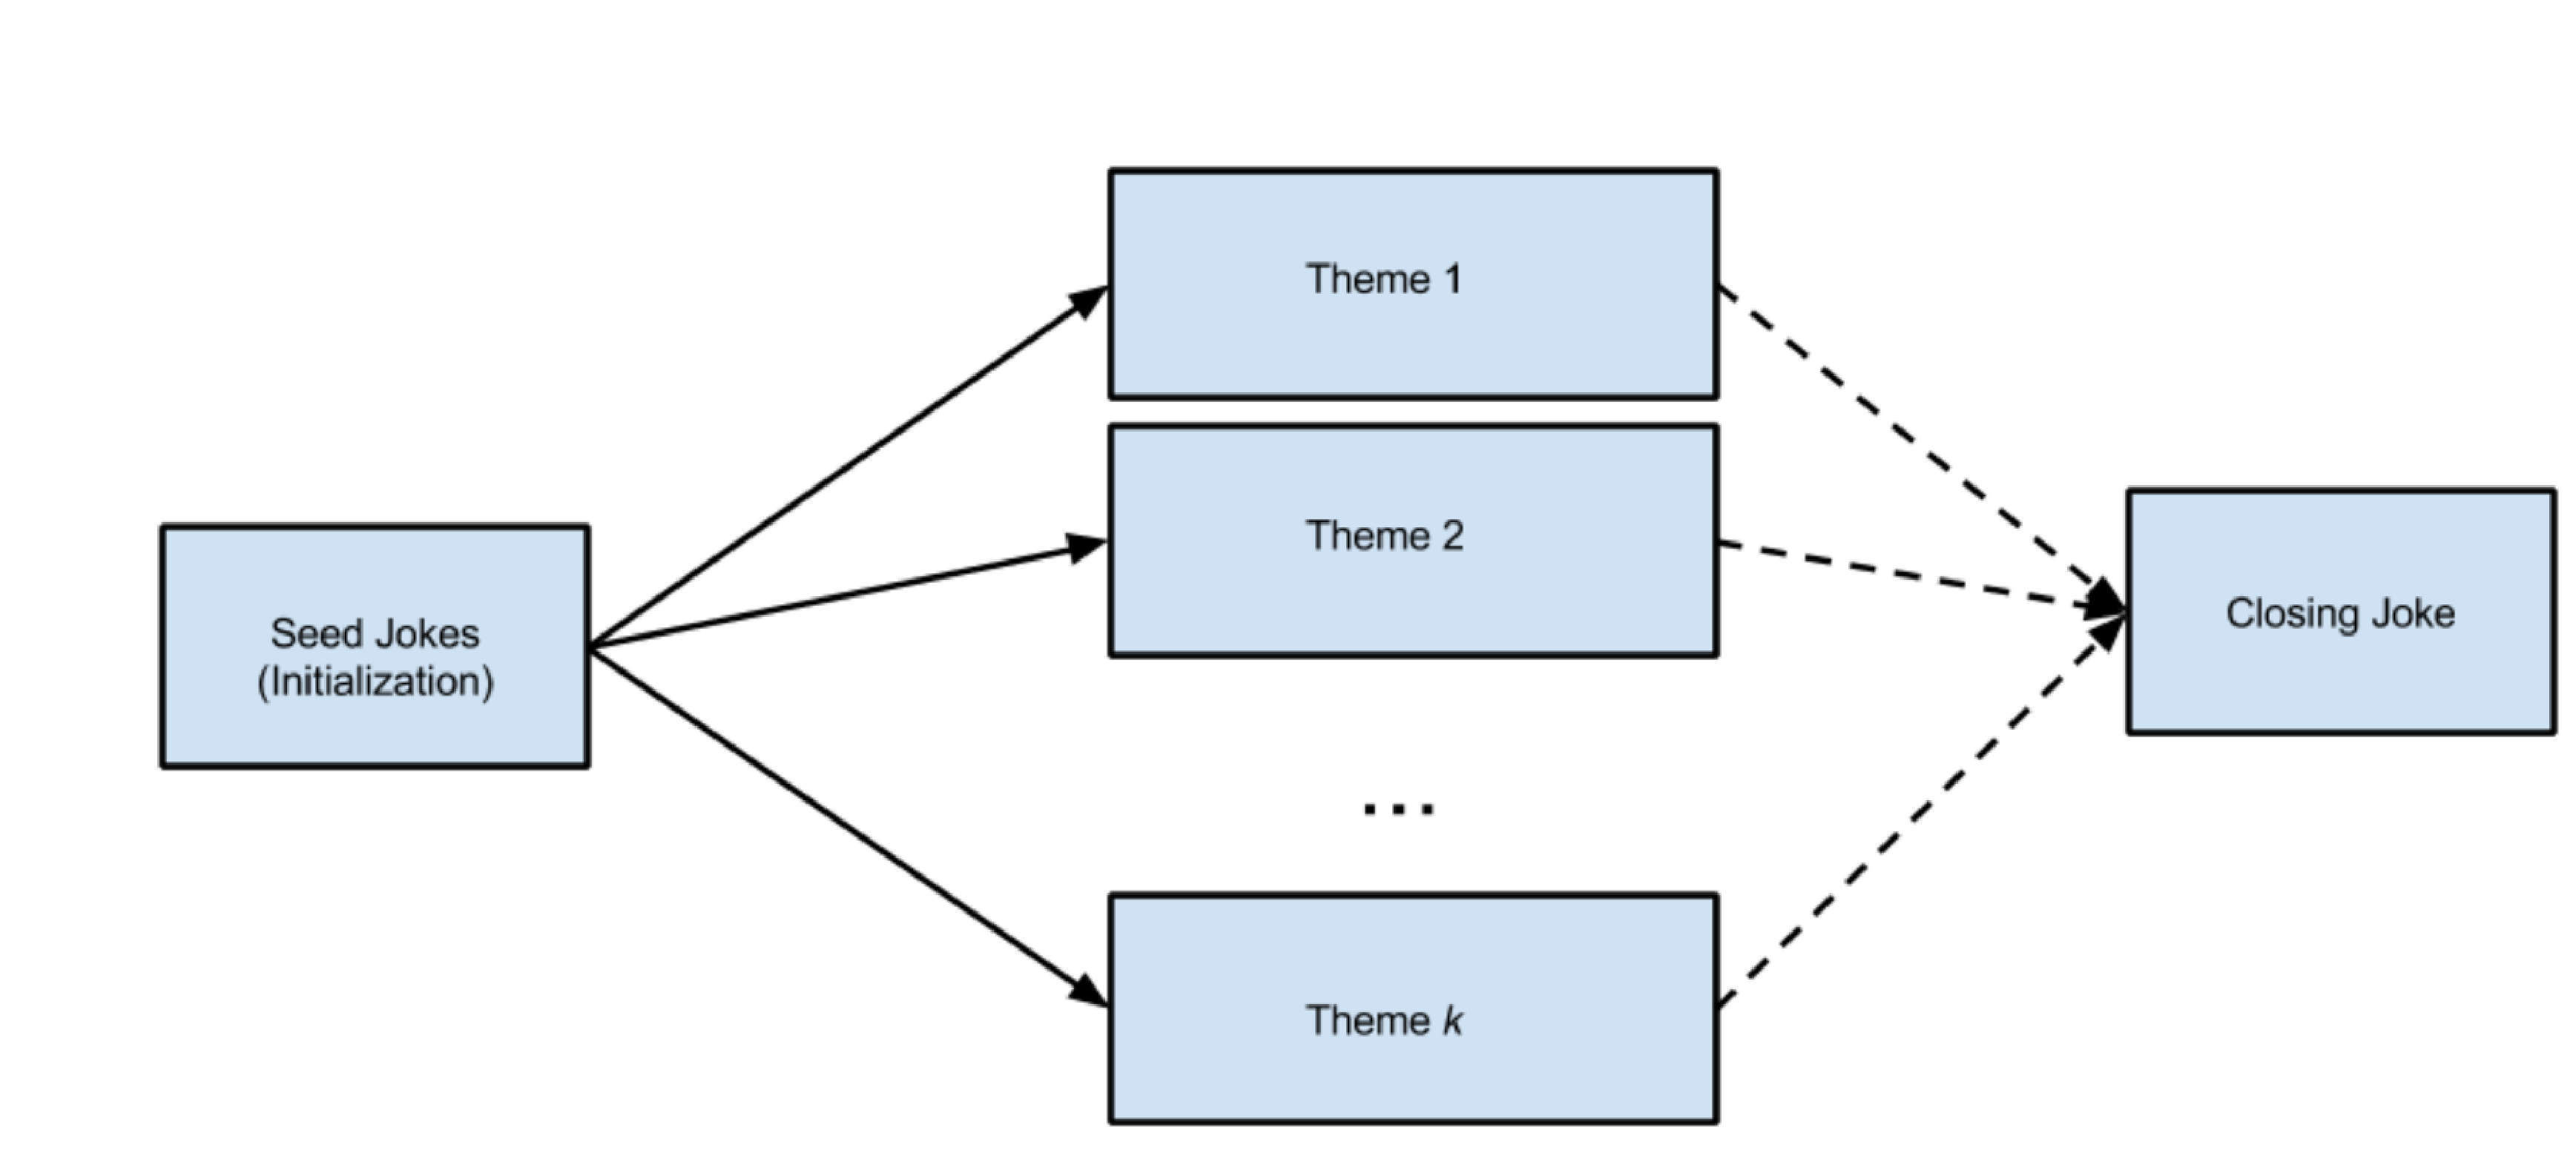
\includegraphics[width=0.75\textwidth,height=0.75\textheight,keepaspectratio]{fig0}
  \caption{This shows how the algorithm will have up to \textit{k} Themes to choose from, determined from the seed joke. The closing joke is a subset of the set of all jokes, and may be outside of a specific theme. There could be different spanning trees of jokes that end at the same closing joke}
  \label{fig:joke}
\end{figure}

In the beginning of the set, the comedian will present an ”initialization” procedure, known
as the ”Seed Jokes” to test the response of the audience to different jokes. Depending on their response, the comedian
will transition to a theme that is evaluated to be the best fit. The robot comedian will have many jokes to choose from
that contain different material, but not all audiences will like all of the jokes. Figure \ref{fig:process} shows how the theme will be
chosen from a set of up to k themes. From the Seed Jokes, one of the themes will be chosen. If there is time, we may also
explore the choice of strategic closing jokes. These jokes might be stronger jokes than some of the others, and is helpful
in ending the show on a stronger note.

For example, if two of the seed jokes are about ”food” and ”Mindfulness”, the performance will branch to the
respective theme that matches the audience response (Branch 1 ”Food” or Branch 2 ”Mindfulness”). If jokes with a
theme of ”food” are not landing with the audience, the algorithm will need to know when to transition to a new theme, or when to end the set. When the robot tells a joke, it needs to be able to analyze the feedback and choose the next joke
to perform. This needs to be done quickly, so that the robot is not spending noticeable time (for the audience) choosing
a joke. There may not be a lot of jokes to choose from, but the choice needs to be made fast.

\begin{figure}[H]
  \centering
  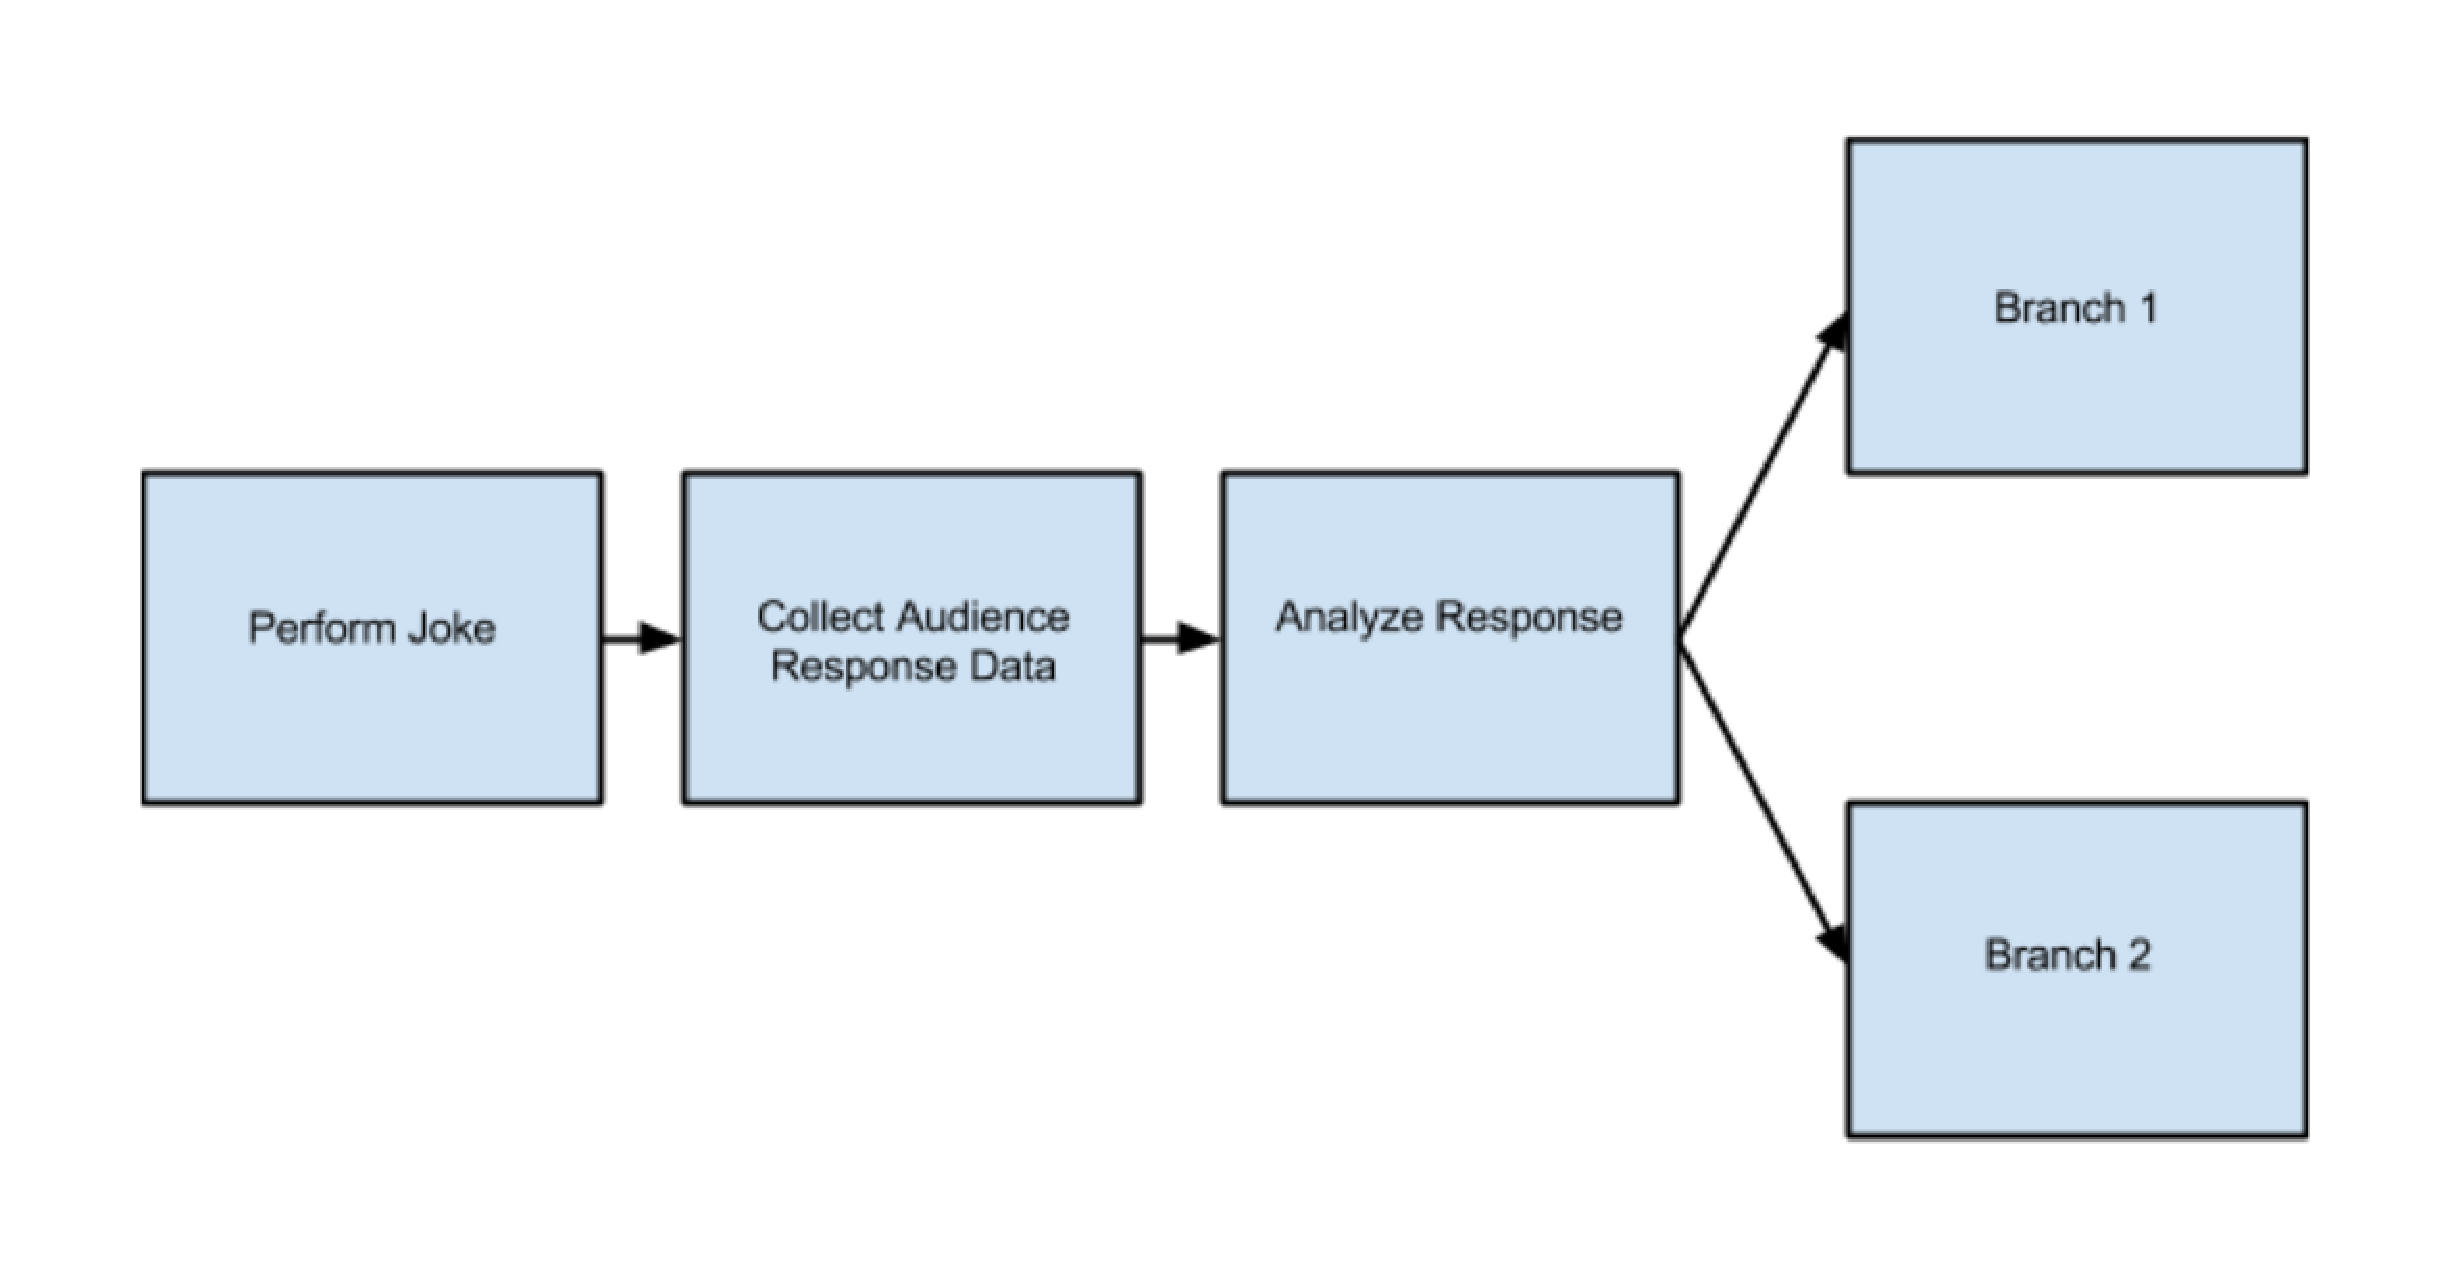
\includegraphics[width=0.75\textwidth,height=0.75\textheight,keepaspectratio]{fig1}
  \caption{ This flow-chart depicts how, once the robot delivers a joke, will wait for feedback, interpret data, and then make a joke decision (Branch 1 and Branch 2)}
  \label{fig:process}
\end{figure}

The close of the robot’s act will include the robot’s report of what attributes the audience
responded to most. The hypothesis here is that getting insight into the robot’s algorithms will increase the audience’s
perception of the robot’s intelligence, and, second, that it will make them laugh. People enjoy hearing about themselves.

All of the above behaviors, from adaptation to the end of performance audience report need to be evaluated with
real people. Initial tests will be done on campus with small groups of people, the final test will be done in conjunction
with the crowd-work and character manipulations, testing the entire algorithm together with a larger crowd, e.g., 10-25
people.


\subsubsection{Crowd-work}
\paragraph{Goals}

Similar to the crowd report described above, we hypothesize that generally interacting with the audience (a.k.a crowd-
work) throughout the performance, will improve the audience’s overall enjoyment of the show. We want to analyze the

importance of this crowd-work relating to the central design of the project. Crowd-work should make the audience feel
like they are a part of the show. This can be done in different ways - calling out and talking to the audience, watching
the audience and incorporating them into the jokes, and asking them questions to keep them engaged, or to build off to
make new jokes.

\paragraph{Methods}
There are various kinds of crowd-work we want to test: one research question is whether crowdwork matters at all, and
the second is does the crowdwork needs to be real or robot can just pretend it is paying attention?

To answer these questions we suggest three research conditions: (1) no crowdwork, (2) fake crowdwork, (3) real
crowdwork. The first one would be no crowd-work whatsoever. The robot goes about performing its set and does
not directly address the audience at all. The second could spanover-the-top and inaccurate crowd-work, or best-guess
crowdwork, with the possibility of being real (e.g., predicting that most people in the audience were from Oregon, even
if it did not hear what they said). The third case would integrate actual robot sensing. It would be important for
conditions \#2 and \#3 to be parallel to assess whether crowdwork really matters.

As condition one is fairly obvious, let us discuss deeper possibilities for condition \#2. In the obviously fake research
condition, the robot will talk to the audience directly but it will be completely wrong in its observation. The absurdity
of a robot trying to understand the audience and being completely off could be entertaining for the audience, or it may
not connect with the audience at all. The exact reception of this sort of crowd-work is something we are trying to study.
The other version of condition \#2 is realistic but premeditated. For example, pre-known facts about the audience
could be built into the robot or guessed. These pre-known facts could include the location of the performance, age
demographics of the audience. For example, if the audience is known to be college-aged, the robot could be fed input
to make comments about things relevant to college students.

Using actual robot sensing data is condition \#3, and is certainly the ideal model, but requires sensing capabilities,
processing power and hardware, so it would be good to know if it is really necessary. In this condition, the robot would
be actually looking for cues from the audience during certain situations. For example, one example is asking questions
and capturing words from the audience, then using that same word later. For example, the robot could ask a simple
question about the weather, or the audience member’s hometown. In this case, the robot can listen for specific words
and ask another question about that specific town or city.

Another real sensing capability the robot could use is audience volume levels after the delivery of jokes. The robot
will keep track of the audience input. The robot could then acknowledge if the audience enjoyed the joke or did not
enjoy the joke using these inputs. Additional sensors and processing abilities on the NAO robot include face-detection
and bumper detection, so the exploration of audience sensing could potentially include speech, volume, vision, and
touch.

All of these conditions will be assessed with live audiences (even if its just a few people in a classroom) to check to
what degree is crowd-work important for a robot comedian. The audience’s response will be used to see if they enjoy
a humanized robot or if they prefer a more robotic one, or maybe even a combination of both. As crowd work is just a
form of human interaction, we expect it will improve the audience’s perception of the robot’s intelligence, add surprise
to the show, and increase audience enjoyment levels. On the other hand, perhaps faking it can get 80% of the effect of
the real version. That will be part of the evaluation.



\subsubsection{Character}
\paragraph{Goal}
The goal of this subsection of the project is to examine whether or not robot comedy can benefit from having jokes delivered
from a robot’s perspective. Our hypotheses are that a robot presenting jokes about technology or being a robot will be
funnier than a human telling the same jokes, and that robots will be less funny than humans at telling jokes from a
human perspective.

In Jerry Palmer's \textit{Taking Humor Seriously}, comic meaning is argued to depend on the interrelated factors of a joke's context and setting, its delivery, the identity of the deliverer, and the audience \cite{Palmer:1993}.
Of specific interest to us are the factors of a joke's delivery and the identity of the deliverer.
In previous studies, robot comedy has been used to analyze effective aspects of joke delivery.
However, little has been done in discovering effective aspects of a joke's content as it relates to the identity of the deliverer.
For example, Sj\"{o}bergh and Araki \cite{RobotsMakeThings:2008} found that jokes were perceived as funnier when delivered by a robot, rather than being delivered in text form.
However, Sj\"{o}bergh and Araki used word-play jokes that were gathered from the internet, and delivered them through a robot by using a flat, machine-like sounding text-to-speech tool called AquesTalk. This form of delivery does not take into account the importance of effective joke delivery. While Sj\"{o}bergh and Araki did not implement measures for analyzing non-verbal delivery, other work has examined the importance of non-verbal signals in delivering jokes \cite{KatevasRobot:2014} \cite{KnightEightLessons:2011}.
Despite this, there is little to no existing literature on the effectiveness of jokes related to the identity of the deliverer.
In our context, this means examining the effectiveness of robot-specific jokes in robot comedy.

\paragraph{Methods}
To address this goal, jokes will be written from a human or robot perspective. The jokes written from a human
perspective will have a corresponding robot version, ideally with as much one-to-one correspondence as possible in
regards to cadence, length of joke, parallel content, similar motions, and so forth. These jokes will be subject to intense
scrutiny by members of the project and by the client, such that revisions and edits can be made to create funny jokes
with a definite correspondence between the two versions. For example, a human version of a joke might look like the
following (lines with a definite correspondence with the robot version are highlighted):

\begin{lstlisting}
Hey, hey, I got news. This is big.
Ok, quiet down. Get this.
That's RIGHT folks.
I'm no longer single. *throws hands up*
(*@  \hl{I met a man on tinder.}  @*)
(*@  \hl{His name's Sebastian. He's a math nerd.}  @*)
(*@  \hl{Swiped right as fast as my fingers could move.}  @*)
\end{lstlisting}

Whereas, the robot version of the above joke is shown below.

\begin{lstlisting}
Hey, hey, I got news. This is big.
Ok, quiet down. Get this.
That's RIGHT folks.
I'm no longer single. *throws hands up*
(*@  \hl{I met a robot on tinder. }  @*)
(*@  \hl{His name's Data.  He's a really geeky robot.}  @*)
(*@  \hl{Swiped right as fast as my motors could turn.}  @*)
\end{lstlisting}

\paragraph{Development process of joke writing}
These jokes will be scripted in Choreographe, where adjustments to vocal tones and pausing will be made.
Then, animating the robot for non-verbal gestures will be done to enhance the delivery.
The overall process may look similar to Figure \ref{fig:write_process}.

\begin{figure}[H]
  \centering
  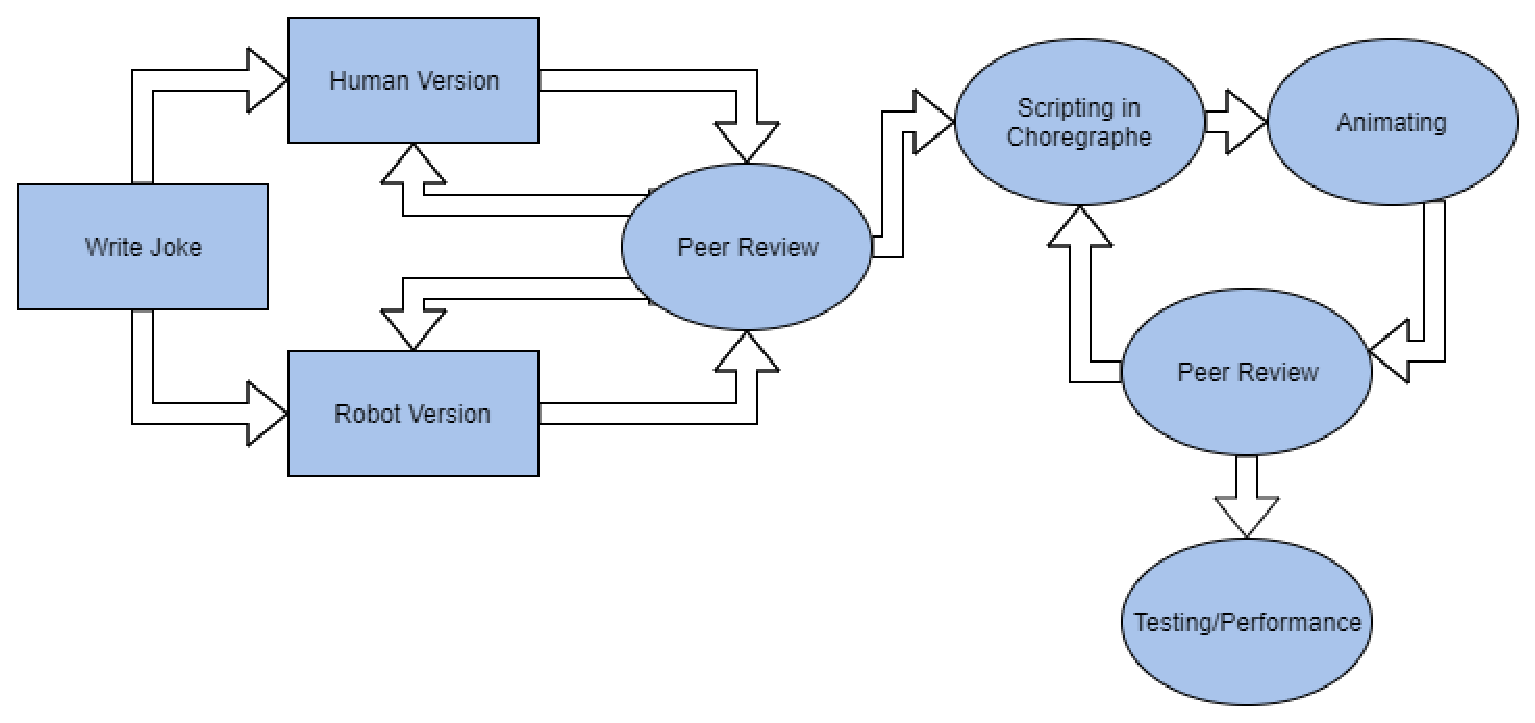
\includegraphics[width=0.75\textwidth,height=0.75\textheight,keepaspectratio]{joke_writing_process}
  \caption{The work flow from joke writing to testing.}
	\label{fig:write_process}
\end{figure}

\paragraph{Experimentation}
The stand-up routine of the robot will comprise of text of the joke themselves, the motions that the robot uses to
accompany them, and the way the robot surveys the audience after each punchline, e.g., in a human or robotic fashion.
To determine the differences in audience response to the routines, studies will be done first on Amazon Mechanical
Turk, and later with co-located audiences. Participants will be shown a video of the robot’s stand-up routine, and then
presented with a short survey. The routines will be between 5 and 10 minutes long, and the survey will include questions
pertaining to each joke or routine. Participants will be compensated with standard rates for watching brief videos and
answering survey questions.

\subsection{Conclusion}
This document overviews our main Robot Comedy research questions, and the three software implementation targets
for the capstone: adaptation, crowd work, and robotic versus human-like character. We hypothesize that all three will
play a role in designing an effective robot comedian.

Designs for the adaptive transitioning algorithm between jokes, the integration of an audience into the performance
of a set, and the exploration of robotic character in joke content and delivery have been described. To evaluate each,
we have described the hypotheses we have and the research conditions we will compare to validate or invalidate them.
People will be the ultimate judge of whether a robot performance will be successful, thus, human evaluations are critical.
This project will use of combination of in-person and video studies to evaluate each research question individually in
the winter term, then bring all parts of the programming together for collective evaluations with larger audiences on
campus in the spring.

In following through with this in the research and development process, we will better understand the role of
acknowledging and interacting with the audience, as well as the robot character itself, if creating experiences between
people and robots, on and off the stage. Not all robots will tell jokes, but understanding more about what people value
in robots could be reused in related robot applications from tour guides to English teachers, or even a factory robot that
delivers parts and lightens a worker’s day by making jokes about her favorite sports team.


\documentclass[onecolumn, draftclsnofoot,10pt, compsoc]{IEEEtran}
\usepackage{graphicx}
\usepackage{url}
\usepackage{setspace}

\usepackage{geometry}
\geometry{textheight=9.5in, textwidth=7in}

% 1. Fill in these details
\def \CapstoneTeamName{		AKA Robotics}
\def \CapstoneTeamNumber{		13}
\def \GroupMemberOne{}
\def \GroupMemberTwo{			Kevin Talik}
\def \GroupMemberThree{}
\def \CapstoneProjectName{		How to Make an Effective Robot Comedian}
\def \CapstoneSponsorCompany{	Oregon State University}
\def \CapstoneSponsorPerson{		Heather Knight}

% 2. Uncomment the appropriate line below so that the document type works
\def \DocType{		%Problem Statement
				%Requirements Document
				Technology Review
				%Design Document
				%Progress Report
				}
			
\newcommand{\NameSigPair}[1]{\par
\makebox[2.75in][r]{#1} \hfil 	\makebox[3.25in]{\makebox[2.25in]{\hrulefill} \hfill		\makebox[.75in]{\hrulefill}}
\par\vspace{-12pt} \textit{\tiny\noindent
\makebox[2.75in]{} \hfil		\makebox[3.25in]{\makebox[2.25in][r]{Signature} \hfill	\makebox[.75in][r]{Date}}}}
% 3. If the document is not to be signed, uncomment the RENEWcommand below
\renewcommand{\NameSigPair}[1]{#1}

%%%%%%%%%%%%%%%%%%%%%%%%%%%%%%%%%%%%%%%
\begin{document}

\bstctlcite{IEEEexample:BSTcontrol}
\begin{titlepage}
    \pagenumbering{gobble}
    \begin{singlespace}
        \hfill 
        % 4. If you have a logo, use this includegraphics command to put it on the coversheet.
        %\includegraphics[height=4cm]{CompanyLogo}   
        \par\vspace{.2in}
        \centering
        \scshape{
            \huge CS Capstone \DocType \par
            {\large\today}\par
            \vspace{.5in}
            \textbf{\Huge\CapstoneProjectName}\par
            \vfill
            {\large Prepared for}\par
            \Huge \CapstoneSponsorCompany\par
            \vspace{5pt}
            {\Large\NameSigPair{\CapstoneSponsorPerson}\par}
            {\large Prepared by }\par
            Group\CapstoneTeamNumber\par
            % 5. comment out the line below this one if you do not wish to name your team
            \CapstoneTeamName\par 
            \vspace{5pt}
            {\Large
                \NameSigPair{\GroupMemberOne}\par
                \NameSigPair{\GroupMemberTwo}\par
                \NameSigPair{\GroupMemberThree}\par
            }
            \vspace{20pt}
        }
        \begin{abstract}
          
          A comedian can observe an audience and improvise a delivery of a joke to connect the audience to the content. This makes the experience more authentic and genuine for the observer. The purpose of this project is to to discover what makes an entertaining interaction by studying a robot that performs comedy. We propose that a performance is enhanced when (1) the comedian interacts spontaneously with the audience, (2) the comedian has and conveys a coherent, well-developed character, and (3) the comedian adapts its act to cater to an audience based on their reaction. This document covers the technical requirements for our project, as well as a description of software, hardware, and outside limitations.

        \end{abstract}     
    \end{singlespace}
\end{titlepage}
\newpage
\pagenumbering{arabic}
\tableofcontents
% 7. uncomment this (if applicable). Consider adding a page break.
%\listoffigures
%\listoftables
\clearpage

% 8. now you write!
\section{Introduction}

  To make an effective robot comedian, we have developed three research questions that will be the basis of three internal systems for the machine. First, we are investigating how spontaneous interactions benefit a set. Second, we want to quantify the benefits of the robot's ability to personify it's character, and lastly how to adapt it's set corresponding to the audiences reaction. My role in this project is to develop an algorithm to adapt the robot's set of jokes based off of audience response.

  Timing and anticipation for jokes are crucial for the success of the set. Every joke that is told provides information to the audience about the robot, and from the opening joke, each new part of the set will build the repertoire of the bot. If a joke is well received by the audience, the relationship between the comedian and the crowd is strengthened, as the people will become more trusting of the content. Every joke will enable the audience to connote decisions, preferences and knowledge of the robot. This is where the connection, otherwise known as the "Theory of Mind", is made with the audience\cite{leslie}.

\section{Individual Role in Project}

Our group will be working collectively to make an effective robot comedian, but I will be specifically working on our third research question: the robots ability to adapt a set based off of audience response. From audience response to a joke, or bit, the algorithm should be able to determine the best fit for the next joke. The bit that tests the audience's preference for humor will be known as the "seed". The seed will be a small subset of jokes that represent the collective set of jokes. For example, the seed bit may have three jokes; one joke could be a self-depreciating joke, one could be a joke about food, and another could be a quick observational joke about the audience. If the audience responded well to the self-depreciating joke, the algorithm should choose the next joke should be at the expense of the robot. 

The seed of the set will give the audience pretense to the performance, and is the introduction of our robot. The delivery of the joke, and the content given has a large impact of robot character, and is out of the scope of the set creation; this is more suited toward the characterization research question. Also, the robot may need a more fluid way to interact with the audience (such as small talk, or crowd-work), which is underneath the breadth of the second research question about audience interaction. My contributions will be towards the system that determines which jokes, from our library of jokes, is best fit for our audience.

The algorithm will need to be able to input the strength of a delivered joke, and return a joke with attributes that match the strength of the joke. This will begin at the seed portion of the algorithm, and pick jokes until the set has lasted 3-6 minutes. The jokes will have some small variability in delivery, that correspond to the tasks of audience interaction and characterization.

\section{Technology overview}
    There have been a couple of previous studies of robot theatre, most notably Dr. Heather Knight \cite{KnightEightLessons:2011}, Katevas et al \cite{KatevasRobot:2014}, and Dr. Guy Hoffman \cite{hoffman2010anticipation}. To accomplish this task of designing an algorithm that can learn from the audiences' response to jokes, it is important to look at previous research, as well as the tools available for accomplishing this task.
\subsection{Previous Work}
  \subsection{ComedyParser}
  Katevas et al \cite{KatevasRobot:2014} has researched a robotic comedian agent previously with some success. During their research, they implemented a program called ComedyParser (https://github.com/minoskt/ComedyParser ) that collects audience response information from SHORE computer vision, and performs the stand up set. The decision components, or what the robot does with information gathered from the SHORE vision, will be most important for implementing an algorithm in our project. 
  A limitation with ComedyParser is that is specifically needs the SHORE vision to operate. SHORE will be too expensive for our project, and we will have to pursue more freely available systems. One solution that we had devised was to interprate the strength of the audience response to buttons on the robot. This will bypass the sensing component of comedy parser, as sensors for creating an audience model are out of the scope of this project.

  \subsection{Anticipation in Robot Theatre}
  Research conducted by Dr. Guy Hoffman studying the implications of anticipatory actions in social robotics \cite{hoffman2010anticipation}. This particular study found that humans working with a robot that can monitor anticipation for an event allows humans to anthropomorphize the robot with more human like attributes. This study uses non-atomic Markov Decision Processes (MDPs) to model the decisions for events. Additionally, Hoffman models anticipation with an impulse-cue situation, where the robot is waiting for an impulse to trigger a specific cue. This is non-deterministic, as the MDP process is modeled around the probability of an event happening.

  This will be helpful to use in our model, as Python, the main programming language for this project, has several implementations for MDPs, and the related automata "Context Free Grammar" (CFG).
\section{Tools}

  \subsection{Programming Languages}
  \subsection{Python}
  \subsection{java}

\section{Libraries}
  \subsection{Natural Language ToolKit}
  \subsection{PyKov: Markov Chains in Python}


\pagebreak


\bibliographystyle{IEEEtran}
\bibliography{refs}

\end{document}



\section{Introduction - Tech Review Anish}
During stand-up comedy, a performer's ability to influence the audience is vital to an entertaining performance. This involves correctly tying together various social signals such as body orientation, gesture, and gaze by both the performers and audience \cite{RobotComedyLab:2015}. Dr. Knight emphasized on the importance of such non-verbal interactions in order to deliver a successful performance \cite{KnightEightLessons:2011}. We want to add to this and incorporate crowd-work and audience interactions throughout the performances in order to help make the performance enjoyable and engaging for the audience.

\section{Individual Role in the Project}
One of the most important aspects of an effective performance is making the audience feel like they are part of the performance at all times. My role is to integrate this crowd-work throughout the performances. It can involve pointing at and talking to the audience which can be scripted, mostly during the intro and outro of the performance. It can be taken further by using sensors that will be triggered by certain audience actions and reactions.

\section{Literature Review}
The timing, frequency, and duration of a gesture relays a lot of information to the spectator. Dr. Knight conducted various performances with a robot, ranging from performing on stage with an audience to pre-mediated collisions with human environments, like "street performances." Over the course of these performances, there were eight major takeaways that will help make a robot performance entertaining. They were:

\subsection{Convey Intentionality}
Using relatable and appropriate gestures help the communication between the robot and the audience. Since these actions can be predicted by the audience, they consider the robot as an entity similar to them. Displaying empathy while performing also boosts the robot's relatability to the audience.

\subsection{No Mind Without Body}
Human expressions are derived from our physicality. Robots can also be capable of leveraging their embodiment to communicate on human terms. It was found that presence of a physical, embodied robot enabled more interaction as well as enjoyment of said interaction for humans. A robot not fully leveraging its physicality ends up losing a significant mode of communication and is also less expressive.

\subsection{Physicality and Motion}
The audience should be able to connect the robot's non-verbal behaviors to the words. The human brain maps the actions it sees on to itself and imagines itself doing it. This helps the audience put themselves in the shoes of the performer.

\subsection{Outward Emotional Communication Trumps Inward Experience}
The inner experience of the performer is trumped by the success of the outward intentionality conveyed. Most robots are designed to enhance, enable, or empower humans. Simplicity and clean physical design is often the clearest way to streamline communication of robot intention.

\subsection{Gulf between Props and Character}
Robots should be considered to be more like agents (entities) and less like props just standing up on stage. Until now, robots have been lacking in that department and there is a significant gap that exists. Robots lack believable and human-like actions. The various aspects of non-verbal communication like gestures have a significant impact on the robot not being considered an object.

\subsection{Good Actors Outweigh Bad Actors}
Multi-robot or human-robot teams have potential to deliver entertaining performances. Human actors can affect the audience's perception of the robot. They can also make up for the robot's unpredictability and lack of control.

\subsection{Acknowledging/Learning}
Human audiences are cognizant of human social behaviors. The audience can provide real time feedback. This feedback can be used to maximize the audience's enjoyment levels. The robot can constantly read these enjoyment levels and update the attributes of audience likes and dislikes. When delivering a joke, the audience should be given enough time to comprehend and process the joke. Starting the next joke early can break the flow and does not give the audience a chance to appreciate the joke and its delivery. The pause could be filled with the robot gazing around at the audience and posing. This helps develop a good rhythm for each joke.

\subsection{Humor Makes People Like the Robot }
Humor is one of the common grounds across all humans. When a robot performs comedy, and is able to match their sense of humor, it helps establish that common ground. If humor can help robot seem like ?one of us', that could be a significant leap to overcome the idea that robots are only props \cite{KnightEightLessons:2011}.


Katevas conducted studies in a similar fashion. His study hypothesized that interactional dynamics should be just as important to the mass interaction involved in performing comedy in front of a live audience. The interactional dynamics involved addressing the audience - including appropriately timed smiles or relevant gestures. The interactional procedures during a performance helps set the tone for the performance.

Robots provide a unique opportunity to experiment with the interactional processes. They can have a consistent routine while modifying the various aspects of delivery - body orientation, gaze, and gesture.

Embodied robots are likely the best way for the robot the catch the audience attention and make the audience pay attention to the robot. The robot used by Katevas et. al was a humanoid robot consisting of a robotic head, two arms with hands, the torso as well as two legs. The head had two rectangular LCD screens for eyes as well as LEDs on cheeks for expression \cite{RobotComedyLab:2015}.

\section{Methods}

Katevas' studies involved two performances. Each performance involved a compere doing the introductions and warming up the crowd for 10 minutes, followed by a human comedian performing for 13 minutes. Right after that, the robot comedian performed for 8 minutes. This format was used to widen the appeal of the event and to set up a stand-up comedy context. Each performance consisted of approximately 50 people in the audience. The sensors used to capture audience reactions and responses got data for approximately 20 people each performance. These sensors looked for various aspects about the audience including gender and age estimation. It also captured facial expressions and categorizing them into percentages of "happy", "sad", "angry", and "surprised". These facial expressions were used to update the audience model.

Punchlines were distinguished using a faster delivery followed by a short pause. The punchline was also followed by a gaze and a smile and sometimes laughter. The duration of the pause was determined by the feedback received from the joke - a longer pause if the audience is still laughing. While using gestures, a gesture pointing to the audience at certain times seemed to get the most positive feedback. The studies found that the enjoyment levels of the audience during the robot performance lied between the compere and the human comedian \cite{RobotComedyLab:2015}.

We could use the dynamic use of sensors to take into account and acknowledge when a delivery was successful or not. We will capture an initial audience model by performing a few "trial" jokes to get a grip on what kind of humor or topics the audience would enjoy. The robot's model for the audience could be acknowledged later to give the audience a feeling that they are being heard. While the sensors in our robot are not sophisticated enough to capture emotions from a crown of people, we will use audio feedback from the audience to update the audience model on the fly.

Dr. Knight's research was more varied. Her performances ranged from stage and audience performances to guerrilla theater performances (street performances). The research looked to add value to developing everyday robots in addition to the entertainment value. It is easy to survey people and learn more about human-robot interaction when there is a significant amount of people present in the audience.

Using the theater context also helps the development of social robots. As noted before, non-verbal expression plays a key role in understanding sociability. A robot's movement and engagement pattern impacts the people's interpretation of the robot's intention, capability, and state. Physical theater provides pre-processed methodologies for interpreting and communicating human non-verbal behaviors that can be portrayed on robots \cite{KnightEightLessons:2011}.

Capturing an audience model is not as feasible when performing guerrilla theater. The audience model would not be very accurate since the crowd is constantly changing. In such situations, the crowd-work would depend on gestures and being able to identify what jokes were successful.

\section{Conclusion}

Humor is one of the major emotions that is common ground for people from all backgrounds. Robots that have a grasp of humor would help bridge the gap present in human-robot interaction and bring people closer to robots. Stand-up performances provide a great platform for the robot to express its humor and show the audience what it is capable of. It will be vital to make the audience feel like a part of the performance, just like most successful stand-up comedians. In order to do this successfully, we need to take a lot from the research done in the past and build upon it.

\section{Introduction - Tech Review Arthur}

This is a tech review for Group 13, written by Arthur Shing, for the project "How to Create an Effective Robot Comedian".
This project is a research project that intends to extend on research done in the field of Human-Robot Interaction.
Our end goal for this project is to create an effective robot comedian that can perform in front of a live audience.
In seeking to create an effective comedian, we hypothesize that comedy scripts with greater degrees of (1) crowdwork, (2) character, and (3) adaptiveness, will create more effective comedy, and have a more positive response from the audience.

\subsubsection{Role}
As for my own role in this project, I am focusing on (2) the effectiveness of coherent character in comedy.
This entails the creation of comedic scripts with varying degrees of character coherency.

\subsubsection{Technologies and Research Design}
In the following subsections, I will explore the options and choices we had for alternative topics for our second research question on (2) character, robots, and SDKs and environments. Unlike the technology used for the other two research questions of (1) crowd work and (3) adaptiveness, implementing character will require fewer pieces of technology. For instance, both of the other variables will require some sort of sensing technology, while the implementation of character will not. Consequently, I had fewer technological features to choose from after research questions were decided. In place of the third piece of technology, I will discuss choices we considered for research questions.


\subsection{Research Questions}
The three research questions our group has decided on are the effectiveness of (1) crowd work, (2) character, and (3) adaptiveness in comedy. As a research project, these questions may be subject to change in the future. In deciding upon these three topics, various limitations were taken into account. In this subsection, I will discuss the decision on (2) character, as well as other topics we considered.

\subsubsection{Comedic Genre as a research topic}
One topic we considered was the effectiveness of different genres of comedy.
This includes genres such as deadpan, black comedy, slapstick, or specialized robot comedy.
The first thing we considered was the feasibility of implementation.
Deadpan comedy would either be the easiest or hardest part of the implementation, depending on the dynamics of the vocal software.
The NAO's software is likely unable to mimic exaggerations in vocal expressions, but its monotonous (although mildly expressive) delivery may give way to a successful deadpan delivery.
Black comedy is likewise feasible, although probably inappropriate for research.
Slapstick humor would be harder to implement, with movement limitations that the NAO robot has.
Similarly, the NAO robot would be limited by its battery life and its tendency to fall over.
Specialized robot comedy is an area of great interest to us.
This genre of comedy might include robot-specific jokes; jokes that only a robot would have the right to make.
For instance, joking about its own programming, motor, or intellectual deficiencies might prove to be effective.


\subsubsection{Dialogical Comedy as a research topic}
Another topic we considered was the effectiveness of two parties in stand-up comedy.
In previous tests done by Heather Knight, it was found that a robot by itself could only maintain the attention of a human audience for 2-3 minutes \cite{OneNote:Anish}.
However, with a human interacting with the robot, this time could be extended to twice or three times as long.
Additionally, studies and research could be taken from ventriloquism.
One example of a successful implementation of a robot comedian in tandem with a stand-up comedian in popular culture is Geoff Peterson from The Late Late Show with Craig Ferguson \cite{GeoffPeterson}.
Peterson acted as a sidekick to Ferguson, and although he had an actual voice actor behind the scenes, Peterson could serve as an example of a goal for this topic.
As for implementation on the NAO bot, most of the dialogue would be prescripted with lengths of time between each line for the human to speak.
Another option would be for the human to hold a remote that activates the robot's next line, although this would seem much more scripted.


\subsubsection{Character as a research topic}
The effectiveness of character design was also a topic under consideration.
In much of early previous work on robot comedy, jokes were simply read off one at a time, resulting in a rigid, static comedic structure \cite{RobotsMakeThings:2008}.
Stand-up comedy, however, seems to thrive off of the buildup before each punchline, as well as the quirkiness of the comedian.
Implementation of this may include writing scripts with varying degrees of character.
Character might involve nonverbal gestures, expressivity, and consistency.
For instance, a script with a high degree of character may mean more pronounced, expressive motions, as well as stronger expressive language.
A script with a moderate degree of character may only include expressive language, or might even employ morose language to portray a different type of character.
On the other hand, a script with a low degree of character may simply ramble off jokes, or speak with a minimal amount of non-verbal language.

\subsubsection{Discussion of Research Topic Ideas}
Overall, we found that the discussion of character as a research topic might prove to be the more fruitful endeavor.
Additionally, aspects of comedic genre could be incorporated into the topic as a subtopic or stretch goal, seeing that certain genres of comedy necessitate certain comedians.
For instance, robot-specific comedy may require a comedian with a consistently dry or self-deprecating character.
Having the effectiveness of character as a research topic gives us more flexibility in adjusting our research questions in the future, as well as a broader range of ideas to draw from.

\subsubsection{Conclusion of Research Topic Ideas}
We will research the effectiveness of character implementation in robot comedy.

\subsection{Robots}
Our project will require a robot as the comedian to conduct testing. This robot ideally has vocal capabilities, as well as gesturing capabilities. The three following robots include both of these capabilities.

\subsubsection{RoboThespian}
The RoboThespian has been implemented in Human-Robot Interaction studies in the past.
It is a humanoid, life-sized robot designed for human interaction in public.
It was used to great success in stand-up comedy performance study done by Katevas et. al \cite{KatevasRobot:2014}.
Additionally, it has been used in other theatrical contexts \cite{Spillikin} to some success.
The RoboThespian is constructed by Engineering Arts, and comes with a touchscreen kiosk for the user that can be used to trigger content, view sensors, and actively engage or control the robot.
For the most part, the RoboThespian uses predefined timed animations in its performances through its stock software \cite{KatevasRobot:2014}.
However, its responsiveness can be optimized in a Python IDE that is provided by Engineering Arts.
The RoboThespian stands at a height of roughly 6\", and weighs 97 lbs including a floor base.
The robot also features pneumatic and DC servo motor actuators for the upper body, upper limbs, and head, including jaw actuation and distinct fingers.
It also has a starting price of \pounds59000 \cite{EngineeredArts}.


\subsubsection{Pepper}
The Pepper robot is a small humanoid robot that was built to perceive and respond to emotions.
Designed by Aldebaran Robotics, the Pepper bot was created to interact as natural and intuitive as possible.
It includes 4 directional microphones on its head, as well as two HD and one 3D camera to locate and identify emotions in voices and faces.
It also comes with six laser sensors, three obstacle detectors, and two ultrasound sensors.
The Pepper robot has also had experience in stage work and has been used in Japan to mild success \cite{PepperVid}.
It specializes in socializing and reacting to perceived emotions.
The robot also comes with a tablet on its chest to supplement human interactivity.
The Pepper weighs in at 62 lbs.
It has a starting price of \$25,000. However, when it was first released, it had a starting price of \$2,000 with a \$300 monthly maintenance fee.
A Pepper SDK for Android was released just this year. \cite{PepperBot}

\subsubsection{NAO robot}
The NAO robot is a humanoid robot featuring upper and lower body joints.
Also designed by Aldebaran Robotics, it has 25 degrees of freedom and multiple sensors for perceiving the environment.
These include 4 directional microphones, as well as two HD cameras for vocal and facial recognition.
The NAO robot was created to be extremely customizable.
It has a small frame, weighing 9.5 lbs.
It has been previously used to study Human-Robot Interaction and comedy by Knight et al. \cite{KnightSavvy:2011}.
The robot can be programmed through a software produced by Aldebaran Robotics, called Choregraphe.
It has a starting price of \$9,500 \cite{BuyNAO}. \cite{NAORobot}

\subsubsection{Discussion of Robots}
The NAO Robot is the most accessible to us, as our client already owns one.
The RoboThespian and Pepper robot have also only recently launched SDKs for development.
This led us to be wary of possible bugs and issues that have not yet been addressed in development.
Our client is also familiar with the development environment for the NAO robot, which will make learning it an easier process.
In addition, the RoboThespian and Pepper robot are priced much higher and lack lower body mobility.
The lower body mobility of the NAO robot may benefit from using non-verbal gestural cues that cannot be done on the other two robots.
These gestures may increase the effectiveness of our comedy \cite{KnightEightLessons:2011}.
The RoboThespian and Pepper Robot are also significantly heavier than the tiny NAO robot, which may impact our efficiency with hands-on programming and transporting the robot.

\subsubsection{Conclusion of Robot Choice}
We decided to use the NAO Robot for our project, based on accessibility and efficiency.

\subsection{SDKs and Environments}
The NAO Robot can be programmed in several different ways and comes with several different SDKs. It uses an API called NAOqi that is available in eight different languages. However, only C++ and Python are supported on the robot, while the others are only supported on the computer for remote access \cite{NAOSDK:Overview}.

\subsubsection{C++}
The C++ framework is the most complete one, and allows a developer to write real-time code at high speeds.
The developer can access specialized proxies, which are optimized and give direct access to existing methods.
These proxies also provide compile-time type checking.
The following is an example of specialized proxy usage.

\begin{lstlisting}[language=C++]
	#include <alproxies/altexttospeechproxy.h>

	const std::string phraseToSay = "Hello world";
	AL::ALTextToSpeechProxy tts("nao.local" , 9559);
	tts.say("Hello world");
\end{lstlisting}

In addition to these optimized proxies, generic proxies can also be used.
With these, methods must be specified by the developer, which may be more prone to err.
These are slower than specialized proxies but can adapt to any module.
This includes user-created modules. User-created method names cannot clash with names bound by ALModule methods.
The following is an example of generic proxy usage. \cite{NAOSDK:C++}

\begin{lstlisting}[language=C++]
	#include <alcommon/alproxy.h>

	const std::string phraseToSay = "Hello world";
	AL::ALProxy proxy("ALTextToSpeech", "nao.local", 9559);
	proxy.callVoid("say", phraseToSay);


	// Or, if the method returns something, you
	// must use a template parameter
	bool ping = proxy.call<bool>("ping");
\end{lstlisting}

Movement programmed in C++ is done by calling the angleInterpolation method under the ALMotionProxy module.
This is used by creating an ALValue::array of target angles and times, and passing them into the method.
The following is an example of using angleInterpolation to move the NAO robot's head.
\begin{lstlisting}[language=C++]
	/**
	* Copyright (c) 2011 Aldebaran Robotics. All Rights Reserved
	*/
	#include <iostream>
	#include <alerror/alerror.h>
	#include <alproxies/almotionproxy.h>

	int main(int argc, char* argv[]) {
		const AL::ALValue jointName = "HeadYaw";
    AL::ALMotionProxy motion(argv[1], 9559);
	 	/** Set the target angle list, in radians. */
    AL::ALValue targetAngles = AL::ALValue::array(-1.5f, 1.5f, 0.0f);
    /** Set the corresponding time lists, in seconds. */
    AL::ALValue targetTimes = AL::ALValue::array(3.0f, 6.0f, 9.0f);
    /** Specify that the desired angles are absolute. */
    bool isAbsolute = true;
    /** Call the angle interpolation method. The joint will reach the
    * desired angles at the desired times.
    */
    motion.angleInterpolation(jointName, targetAngles, targetTimes, isAbsolute);
  	exit(0);
	}

\end{lstlisting}



\subsubsection{Python}
The Python framework is the second most complete, and allows a developer to run embedded code.
Unlike C++, Python does not have two different kinds of proxies.
However, methods can be directly accessed once an ALProxy is set to a module.
The Python API allows a developer to use all of the C++ API from a remote machine.
We can infer that this includes user-created modules.
Programming movement in Python is also done by calling the angleInterpolation method under the ALMotion proxy.
Unlike C++, Python does not require the usage of AL::ALValue::array, and uses its built-in lists.
The following is an example of moving the NAO robot's knee in Python. \cite{NAOSDK:Python}
\begin{lstlisting}[language=Python]
	import sys
	import math
	from naoqi import ALProxy

	def main(robotIP):
    motionProxy = ALProxy("ALMotion", robotIP, 9559)
    # KneePitch angleInterpolation
    # Without Whole Body balancer, foot will fall down
    names      = ["LKneePitch", "RKneePitch"]
    angleLists = [ [0.0, 40.0*math.pi/180.0], [0.0, 40.0*math.pi/180.0]]
    timeLists  = [ [5.0, 10.0], [5.0, 10.0]]
    isAbsolute = True
    motionProxy.angleInterpolation(names, angleLists, timeLists, isAbsolute)

	if __name__ == "__main__":
    robotIp = "127.0.0.1"
    main(robotIp)

\end{lstlisting}

\subsubsection{Choregraphe}
Choregraphe is a multi-platform desktop application that is designed to create and test animations and behaviors.
Unlike an SDK, Choregraphe allows for development with significantly less coding involved.
All of the NAOqi API is accessible in Choregraphe, and animations can be done in an intuitive way.
Each joint of the NAO robot can be virtually manipulated in a control console. Figure \ref{fig:choregraphe-movement} shows the ways that the left arm of the robot might be manipulated in the console.
These manipulations require no coding and allow for quick and intuitive viewing of movement options.

\begin{figure}[H]
	\centering
	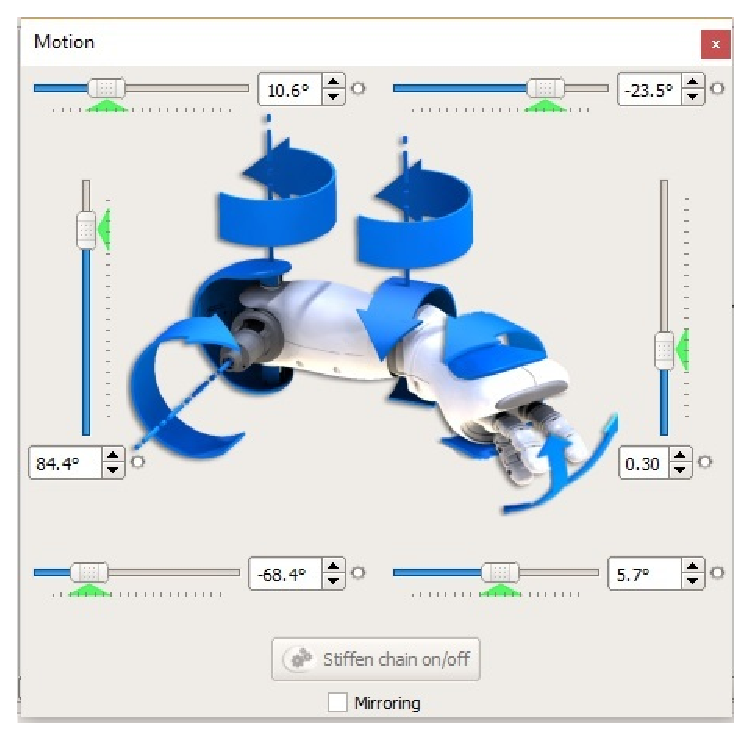
\includegraphics[width=0.5\textwidth]{choregraphe-movement}
	\caption{The motion box in Choregraphe allowing for joint manipulation in the left arm.}
	\label{fig:choregraphe-movement}
\end{figure}

Choregraphe can also connect to an actual or virtual NAO robot as shown in Figure \ref{fig:choregraphe-robot}, allowing programs to be run on the spot.

\begin{figure}[H]
	\centering
	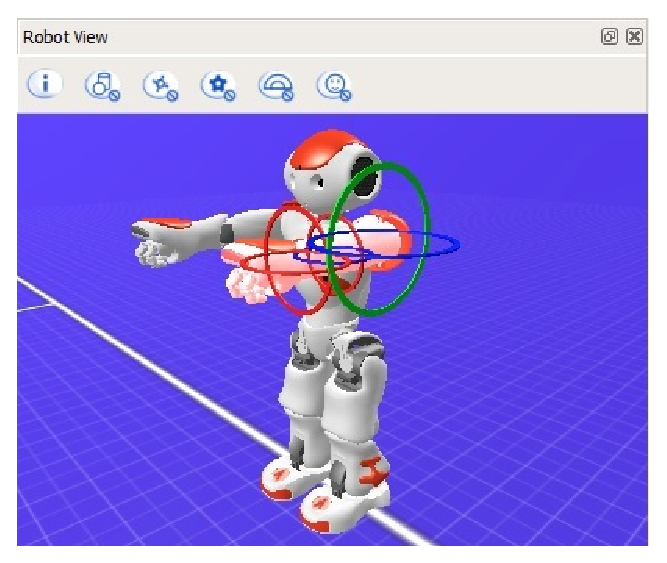
\includegraphics[width=0.5\textwidth]{choregraphe-robot}
	\caption{The virtual robot in Choregraphe. In this image, the left arm can be manipulated.}
	\label{fig:choregraphe-robot}
\end{figure}

Animations can also be created in tandem with vocalizations using a timeline feature, as shown in Figure \ref{fig:choregraphe-timeline}. This feature allows a developer to choose the frames at which the NAO robot will position itself, as well as the words that will be spoken while doing so. \cite{NAOSDK:Choregraphe}

\begin{figure}[H]
	\centering
	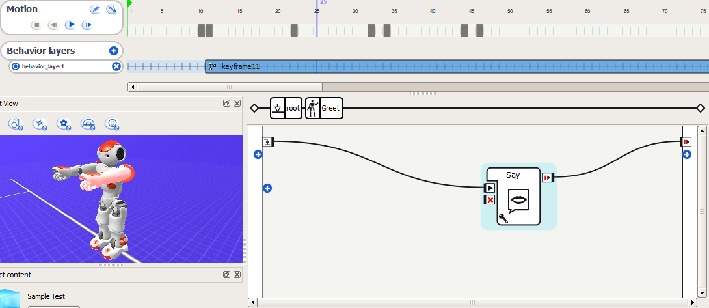
\includegraphics{choregraphe-timeline}
	\caption{The Choregraphe environment. In this image, the timeline is being manipulated for animations along with vocalizations.}
	\label{fig:choregraphe-timeline}
\end{figure}

\subsubsection{Discussion of SDKs and Environments}
While the C++ and Python SDKs are comprehensive and well made, for my purposes, animations and dynamic actions are a greater focal point.
Because of this, Choregraphe seems like the ideal environment for the research question of the effectiveness of character.
As most tests will involve predetermined scripts and little sensor usage, movement will be a vital part of conveying certain character traits. This will be most efficiently done in Choregraphe.

\subsubsection{Conclusion of SDK and Environment Choice}
For our purposes, Choregraphe will be used to program the robot.


\section{Weekly Blogs}

\subsection{Kevin Talik}
	\subsubsection{Fall Term}
	\begin{itemize}
		\item{Week 1-2} \\
			Got project this week; Problem statement due October 10; email client and team . 
			We set up a slack channel ( akarobotics.slack.com ), and shared our availability. 
		\item{Week 3} \\
			We need to come up with a proposed solution that is specific enough for us to define what we intend to fix, but vague enough so that we can have some room for exploration (as this is a research project). 
			We need to make sure that our problem statement reflects that stand up comedy is a metaphor for human to computer interaction. 

		\item{Week 4} \\
		Make sure github is organized and easy to understand for Kirsten and Ben. 
		LaTeX Font, IEEE standard font for the first page. Sans-serif not serif 
		\item{Week 5}
			\begin{itemize}
				\item \textbf{Plans} \\
				Finish Scripts for local, remote and real world. 
				Explain research questions in scripts 
				Practice the nltk and choreograph 
				\item \textbf{Problems} \\
				Kirsten gave us a 92 on the problem statement, she is having difficulty understanding our research based goals. 
				\item \textbf{Progress} \\
				We are behind on the requirements, and need to focus on how this assignment will drive the research for the project.
				We need to focus on documentation quite a bit as well. Improve notes
				\item \textbf{Summary} \\
				Meet with Kirsten to help elaborate on research deliverables.  
				Organize research, look up ieee research. 
			\end{itemize}

		\item{Week 6}
			\begin{itemize}
				\item \textbf{Plans} \\
			Kirrsten is looking at our rough draft right now, and there will also be a rubric for the final that we can look at.
			Research Class this week. We talked about:What are you trying to solve? Can a robot dynamically interact to a crowd? Robot Character perceivable to audience? Adaptive content based from audience feedback?
				
				\item \textbf{Problems} \\
				Expectations are a medium concern. Research based work is something we dont have to worry about without an IRB.
				\item \textbf{Progress} \\
				
					Ben mentioned that our project is difficult, and is masters and PhD level work. Mcgrath and Kirsten are meeting with Heather to make sure that we have a reasonable amount of that can be completed during this school year. 
				\item \textbf{Summary} \\
					Our secondary objectives are going be structured around the dynamic nature of the crowd adaption. If we can come up with a clever solution to implement decision and dialogue choices, we can add it into our design of the machine, but we use the machine to perform the research 
				
			\end{itemize}

		\item{Week 7}
			\begin{itemize}
				\item \textbf{Plans} \\
				Tech review, look at technology for language processing.
				\item \textbf{Problems} \\
				ipsum
				\item \textbf{Progress} \\
				Markov Decision Process, MDP 

				https://www.cs.rice.edu/~vardi/dag01/givan1.pdf 

				Pykov, markov chains in Python  

				https://github.com/riccardoscalco/Pykov 

				A way to make state machine with probability transitions, based off of obvservations 
				\item \textbf{Summary} \\
				Further Designed ways for crowd to receive input.ould test with a couple people yelling at a robot, to test what high audio levels do to the input 
			\end{itemize}

		\item{Week 8}
   			\begin{itemize}
				\item \textbf{Plans} \\
				Use tech review as both tech and literature review. Make sure that my choice of tools is unbiased. None of the "i did it because i did it" sort of things.
				\item \textbf{Problems} \\
				Current view of the tech does not describe the technology well with the features.
				\item \textbf{Progress} \\
				Added more AI reviews of tech that I can use:
				Tensor Flow, pytorch, pykov, NLTK, CFG.
				\item \textbf{Summary} \\
				Looked at feedback methods of audio sensors, and AI tools. Language processing may fall out of scope. Its a lot of data.
				Use timelines to implement jokes, break jokes into one sentence in each box, put waits and ambient movement in each joke. Make two timeline boxes to vary the joke\_robot and joke\_human 
			\end{itemize}
		\item{Week 9}
			\begin{itemize}
				\item \textbf{Plans} \\
			testt Say and branching dialogue in choregraphe 
				\item \textbf{Problems} \\
					Organizing large choregraphe functions (timelines are going to be better for things that depend on time, obviously you dunce) 			
				\item \textbf{Progress} \\
			Got say boxes and branching to work, but in a messy way	
				\item \textbf{Summary} \\
				Movements and jokes are going to be best implemented in choregraphe. Algorithm may work by just taking text input, returning text input and the branches just follow the path
			\end{itemize}
		\item{Week 10}
				\begin{itemize}
				\item \textbf{Plans} \\
				Finish progress report
				\item \textbf{Problems} \\
				We should be worried about the progress report, just because it is a lot of work due in a short time.
				\item \textbf{Progress} \\
				Finished Progress report, wrote some comedic devices for comedy. Like, observational humor, Jobs jokes, like uber driver, dance lessons, unemployment
				\item \textbf{Summary} \\
				Further looked at types of jokes, finished Progress report
			\end{itemize}
	\end{itemize}
	\subsubsection{Winter Term}
	\begin{itemize}
		\item{Week 1}
			\begin{itemize}
				\item \textbf{Plans} \\
				Meet with heather, plan implementation term.
				\item \textbf{Problems} \\
					Branching will have to be done in choreographe, does not test well this way (in a physical manner)
					Hand drawn picture notes are hard to put into one note.
				\item \textbf{Progress} \\
				Heather called me the glue, Arthur the Lead voice, and Anish the perception lead.
				\item \textbf{Summary} \\
				For crowd work, look at Bill Burr getting heckled by a blind guy.

			\end{itemize}
		\item{Week 2}
			\begin{itemize}
				\item \textbf{Plans} \\
				Look at Bayes Classification
				\item \textbf{Problems} \\
				More specific so that we can work on improving parts. If I write jokes, they cant be for fun, they have to be specific to the research. 
				\item \textbf{Progress} \\
				Layed out different types of Adaptation. Correct adaptation, incorrect adaptation, and random adaptation.
				\item \textbf{Summary} \\
				Crowd report needs tons of qualities, yet it cant be a joke. Crowd needs to feel like robot is talking to them
				Categories of Jokes, categories of attributes, physicality, appropriateness of the audience.
			\end{itemize}
		\item{Week 3}
			\begin{itemize}
				\item \textbf{Plans} \\
				Meet with team in person to discuss how we will implement our comedian system
				\item \textbf{Problems} \\
				Our Sections are being completed, but they arent co-mingling because we made them alone, and didnt test together.
				\item \textbf{Progress} \\
				Formalized the Break a leg joke.
				Looked at pirate types of job jokes.
				Read about prosodic phrasing to time the jokes better.
				\item \textbf{Summary} \\
			Each of us are struggling with research goals and expectations, 

			and even though we can cover more ground by covering different topics, we 

			are not always on the same page with what each other are doing. 
			\end{itemize}
		\item{Week 4}
			\begin{itemize}
				\item \textbf{Plans} \\
				Writing more jokes for the robot.
				look at adaptation use cases
				\item \textbf{Problems} \\
				Romance jokes are funny, but not appropriate most of the time.
				"Things you can say about your router but not your girlfriend"

				\item \textbf{Progress} \\
				premise writing: Ginger has six fingers and cant work any job that requires hands. Maybe Ginger had a long term relationship with a slow cooker. Had a hot and steamy relationship with a dishwasher. Ginger being a DJ job. "I guess I am doing well at parking, because someone left a note on my car that said 'parking fine'"
				\item \textbf{Summary} \\
				Ginger takling is not as funny as ginger moving.
			\end{itemize}
		\item{Week 5}
			\begin{itemize}
				\item \textbf{Plans} \\
				Work on Bayes Net, implementing AL memory functionality of choreographe, finish haikubot.py
				\item \textbf{Problems} \\
				Heather left the country with the robot without telling us.
				\item \textbf{Progress} \\
					Made a random poem generator from books by HP lovecraft:

					Here are some examples:

		Still more I scraped, and then on some level beach. 

		It is still extant. 

		He had not memorized. 


		-----

		About the period of this material I cannot hope to understand. 

		Of genuine blood there was no whitish deposit whatever. 

		Night would soon fall, and it can't multiply. 

		-----

		Carrington Harris, last of the visible ritual. 

		I had witnessed things more potent than luminosity. 

		It was no one in Yog-Sothoth. 

		-----

		Now the irony is seldom absent. 

		He reeled, and would have let him live permanently with Peleg. 

		Man rules now where They shall break through again. 

				\item \textbf{Summary} \\
				Text generation is funny, need to look more at bayes 
			\end{itemize}
		\item{Week 6}
			\begin{itemize}
				\item \textbf{Plans} \\
				Look further into prosdy, Write more on midterm design.
				\item \textbf{Problems} \\
				The visible scope of choreographe blocks has a terrible implementation, and our behavior functions are unpredictable at this point.
				\item \textbf{Progress} \\
			Prosody, or intonation is the rhythm and emphasis of a sentence. 

			 

			You know. \textit{I} don’t. \ So don’t ask me.

			You know. I \textit{don’t}. \ As a matter of fact, I really don’t.

			You \textit{know} I don’t. \ You know that I don’t.
				\item \textbf{Summary} \\
				Joke Inventory: 2 carbon dating jokes, 2 dial up jokes, 1 break a leg joke, 2 last term random jokes, Autonomous car joke. We are launching jokes from one file, as to look like one performance.
			\end{itemize}
		\item{Week 7}
			\begin{itemize}
				\item \textbf{To do} \\
					Write Break a leg bit, get joke obbject to put into queue.
				\item \textbf{Progress} \\
					Finalized the break a leg joke, got a global queue for jokes initializing. Anish has head tracking implemented. Got a queue working for this.
				\item \textbf{Problems} \\
					Choreographe has a clunky mechanism for writing custom made objects, and python script boxes dont exit flow correctly
			\end{itemize}
		\item{Week 8}
			\begin{itemize}
				\item \textbf{Plans} \\
				Read more about the theory of chatbots. Think: Does showing a character make it more funny, because its showing true to itself?
				\item \textbf{Problems} \\
				Midterm Week, team is busy
				\item \textbf{Progress} \\
				Read this: https://apps.worldwritable.com/tutorials/chatbot/
				\item \textbf{Summary} \\
				Read about the first chatbot from Joseph Weizenbaum.
				I love this quote:
				“It is said that to explain is to explain away. This maxim is nowhere so well fulfilled as in the area of computer programming, especially in what is called heuristic programming and artificial intelligence…Once a particular program is unmasked, once its inner workings are explained in language sufficiently plain to induce understanding, its magic crumbles away; it stands revealed as a mere collection of procedures, each quite comprehensible. The observer says to himself, I could have written that.” 

				—Joseph Weizenbaum, ELIZA (1966) 

			\end{itemize}
		\item{Week 9}
			\begin{itemize}
				\item \textbf{Plans} \\
				Work with anish to get sound report
				\item \textbf{Problems} \\
				Anish could not meet to get sound report working
				\item \textbf{Progress} \\
				Not much progress, audience adaptation is spoofing in bayes net
				\item \textbf{Summary} \\
				we need to meet more frequently in person, 
			\end{itemize}
		\item{Week 10}
			\begin{itemize}
				\item \textbf{Plans} \\
				Identify matching and subscribing to events on naoqi API. Work on final report for winter term
				\item \textbf{Problems} \\
				naoqi API is not used very frequently, making documentation sparce and difficult to understand
				\item \textbf{Progress} \\
				Got final report done for winter.
				Figured out how to wait for behaviors (processes) to finish. Its a busy loop, it uses a lot of power on the robot.
				This will keep checking if the "behavior ended" function call is put into ALmemory 
			\end{itemize}
	\end{itemize}

	\subsubsection{Spring Term}
	\begin{itemize}
		\item{Week 1}
			\begin{itemize}
				\item \textbf{Plans} \\
				\item \textbf{Progress} \\
				\item \textbf{Problems} \\
				\item \textbf{Summary} \\
			\end{itemize}

		\item{Week 2}
			\begin{itemize}
				\item \textbf{Plans} \\
				\item \textbf{Progress} \\
				\item \textbf{Problems} \\
				\item \textbf{Summary} \\
			\end{itemize}

		\item{Week 3}
			\begin{itemize}
				\item \textbf{Plans} \\
				\item \textbf{Progress} \\
				\item \textbf{Problems} \\
				\item \textbf{Summary} \\
			\end{itemize}

		\item{Week 4}
			\begin{itemize}
				\item \textbf{Plans} \\
				\item \textbf{Progress} \\
				\item \textbf{Problems} \\
				\item \textbf{Summary} \\
			\end{itemize}

		\item{Week 5}
			\begin{itemize}
				\item \textbf{Plans} \\
				\item \textbf{Progress} \\
				\item \textbf{Problems} \\
				\item \textbf{Summary} \\
			\end{itemize}

		\item{Week 6}
			\begin{itemize}
				\item \textbf{Plans} \\
				\item \textbf{Progress} \\
				\item \textbf{Problems} \\
				\item \textbf{Summary} \\
			\end{itemize}

		\item{Week 7}
			\begin{itemize}
				\item \textbf{Plans} \\
				\item \textbf{Progress} \\
				\item \textbf{Problems} \\
				\item \textbf{Summary} \\
			\end{itemize}

		\item{Week 8}
			\begin{itemize}
				\item \textbf{Plans} \\
				\item \textbf{Progress} \\
				\item \textbf{Problems} \\
				\item \textbf{Summary} \\
			\end{itemize}

		\item{Week 9}
			\begin{itemize}
				\item \textbf{Plans} \\
				\item \textbf{Progress} \\
				\item \textbf{Problems} \\
				\item \textbf{Summary} \\
			\end{itemize}

		\item{Week 10}
			\begin{itemize}
				\item \textbf{Plans} \\
				\item \textbf{Progress} \\
				\item \textbf{Problems} \\
				\item \textbf{Summary} \\
			\end{itemize}

	\end{itemize}

	\pagebreak


\subsection{Anish Asrani}
	\subsubsection{Fall Term}
	\begin{itemize}
		\item{Week 1-2}
			\begin{itemize}
				\item \textbf{Plans} \\
				Get in touch with client and figure out a good time to meet them.
				\item \textbf{Problems} \\
				Finding a suitable time to work for everyone including the client (minor problem).
				\item \textbf{Progress} \\
				Got in touch with teammates. We set up a Slack channel to communicate going forward. 
				\item \textbf{Summary} \\
				Researched many of the projects that I was interested in. Met with Dr. Heather Knight and discussed the scope of her project and got a better idea about it. It definitely seems like an exciting one. Briefly discussed Dr. Mike Bailey's project with him. After lots of consideration and thinking, decided the top 5 projects. Now all that is left is stay put and be anxious until the projects are assigned. 
				We ended up finding a weekly meeting time with the client. Started working on the problem statement.  We will definitely get a much better idea after we meet our client. 
			\end{itemize}
		\item{Week 3}	
			\begin{itemize}
				\item \textbf{Plans} \\
				Work on finishing problem statement.
				\item \textbf{Problems} \\
				Nothing crazy. Just putting all the info we have in words.
				\item \textbf{Progress} \\
				Working on problem statement with my group.
				\item \textbf{Summary} \\
				Met with Heather Knight. Got a lot of information to work with.
			\end{itemize}
		\item{Week 4}
			\begin{itemize}
				\item \textbf{Plans} \\
				TA Meeting and client meeting. Get familiar with Choregraphe. Work on Problem Statement. Research HRI and humor.
				\item \textbf{Problems} \\
				Finding specific papers on robot performances. See what works in humor/what doesn’t. Aspects that make robots more "human"

				\item \textbf{Progress} \\
				Got a bunch of resources from Heather. Body language improves performance. Improved the problem statement significantly
				\item \textbf{Summary} \\
				Interesting meeting and got a lot to work with. We managed to get a fair amount of research about robots and performances. We need to find an appropriate way to link them both. 
				We finished a draft that Heather did not approve. We made a good amount of changes and supported our claims. This should be improved this week.
			\end{itemize}
		\item{Week 5}
			\begin{itemize}
				\item \textbf{Plans} \\
				Write jokes. Get familiar with Choregraphe.
				\item \textbf{Problems} \\
				Writing scripts can be hard. Defining some aspects of our requirements
				\item \textbf{Progress} \\
				Got some ideas for jokes. Made some progress on requirements
				\item \textbf{Summary} \\
				Went over humor at the meeting and saw potential scripts for the robot that we wrote. Worked on the requirements draft. Discussed our problem statement paper and shared what we are doing with Kirsten. Need to continue working on the requirements doc and make a simple choregraphe program over the weekend. 
			\end{itemize}
		\item{Week 6}
			\begin{itemize}
				\item \textbf{Plans} \\
				Work on requirements. Learn choregraphe
				\item \textbf{Problems} \\
				Finding balance in the requirements doc. Research requirements are hard to predict.
				\item \textbf{Progress} \\
				Made a basic set on Choregraphe.
				Wrote significant parts of requirements.
				\item \textbf{Summary} \\
				The week was alright. Some confusion about the requirements due to the research we are trying to do. Overall, there is more clarity than before which is only going to improve over the weeks. 
We managed to write some content for the requirements subject to Heather's approval. 
			\end{itemize}
		\item{Week 7}
			\begin{itemize}
				\item \textbf{Plans} \\
				Analyze technology and literature reviews.
				\item \textbf{Problems} \\
				Figuring out specific technologies we are using, clarifying requirements further.
				\item \textbf{Progress} \\
				Got some good research to help us get started into the depth of things.
				\item \textbf{Summary} \\
				Met the robot. It was great. Discussed our individual research questions. Got a rundown of previous code.
			\end{itemize}
		\item{Week 8}
			\begin{itemize}
				\item \textbf{Plans} \\
				Learn about sensors in the NAO. Research for lit review.
				\item \textbf{Problems} \\
				Hard to test sensors without access to robot. Limited time with bot.
				\item \textbf{Progress} \\
				Found interesting research about HRI.
				\item \textbf{Summary} \\
				Nothing crazy. Work on paper. Learn more software.
			\end{itemize}
		\item{Week 9}
			\begin{itemize}
				\item \textbf{Plans} \\
				Learn more choregraphe. Make scripts. Account for pauses during performance
				\item \textbf{Problems} \\
				Animating the robot can take a lot of time.
				\item \textbf{Progress} \\
				Getting the hang of choregraphe.
				\item \textbf{Summary} \\
				Thanksgiving dinner was great.
			\end{itemize}
		\item{Week 10}
			\begin{itemize}
				\item \textbf{Plans} \\
				Work on progress report and script.
				\item \textbf{Problems} \\
				Design document and progress report within a few days
				\item \textbf{Progress} \\
				Record footage, wrote scripts
				\item \textbf{Summary} \\
				Recordings, scripts, meetings, papers = dead week
			\end{itemize}
	\end{itemize}
	\subsubsection{Winter Term}
	\begin{itemize}
		\item{Week 1}
			\begin{itemize}
				\item \textbf{Plans} \\
				Get back in the flow of things for winter. Play around with robot.
				\item \textbf{Problems} \\
				Not a whole lot this week.
				\item \textbf{Progress} \\
				Made a few animations and script
				\item \textbf{Summary} \\
				Not a whole lot but warm up to the robot after it was away for all of winter break
			\end{itemize}
		\item{Week 2}
			\begin{itemize}
				\item \textbf{Plans} \\
				Write/execute jokes. Improve design doc
				\item \textbf{Problems} \\
				Writing jokes can be hard
				\item \textbf{Progress} \\
				Got a few joke ideas.
				\item \textbf{Summary} \\
				Churn out jokes - keep working on experiment (IRB) draft)
			\end{itemize}
		\item{Week 3}
			\begin{itemize}
				\item \textbf{Plans} \\
				Similar to last week. Write jokes. Improve doc.
				\item \textbf{Problems} \\
				Joke writing.
				\item \textbf{Progress} \\
				Slow but steady progress.
				\item \textbf{Summary} \\
				More paperwork for design document.
			\end{itemize}
		\item{Week 4}
			\begin{itemize}
				\item \textbf{Plans} \\
				Explore sensors further.
				\item \textbf{Problems} \\
				Hard to test and predict how robot will behave in different environments.
				\item \textbf{Progress} \\
				Got a sound tracking system working that still needs more testing
				\item \textbf{Summary} \\
				Executed an sound following module on the robot. The robot now turns its head toward wherever a sound is coming from. Useful for crowd work.
			\end{itemize}
		\item{Week 5}
			\begin{itemize}
				\item \textbf{Plans} \\
				Poster, progress vid, try using NAOqi SDK.
				\item \textbf{Problems} \\
				NAOqi SDK is hard to work with.
				\item \textbf{Progress} \\
				Worked on some scripts for facial recognition.
				\item \textbf{Summary} \\
				Collaborated on some robot scripts - worked on poster draft.
			\end{itemize}
		\item{Week 6}
			\begin{itemize}
				\item \textbf{Plans} \\
				Focus on midterm report/video.
				\item \textbf{Problems} \\
				Recording and getting robot footage takes time.
				\item \textbf{Progress} \\
				Video went alright.
				\item \textbf{Summary} \\
				Did midterm report. Record/edit videos - churn out content
			\end{itemize}
		\item{Week 7}
			\begin{itemize}
				\item \textbf{Plans} \\
				Understand sensors and API usage.
				\item \textbf{Problems} \\
				Integrating sensors with other animations can break the animations.
				\item \textbf{Progress} \\
				Head/sound tracking works if there are no keyframes stored in head
				\item \textbf{Summary} \\
				Working further on using crowd work components like comparing volume levels from the API.
			\end{itemize}
		\item{Week 8}
			\begin{itemize}
				\item \textbf{Plans} \\
				Communicate with the robot from local computer.
				\item \textbf{Problems} \\
				Compatibility issues with OSX and Python versions.
				\item \textbf{Progress} \\
				Trying different Python installations. It was hard to work with.
				\item \textbf{Summary} \\
				Learned about QiMessaging - communicating with the robot and parsing values
			\end{itemize}
		\item{Week 9}
			\begin{itemize}
				\item \textbf{Plans} \\
				Audio level sensing from the API.
				\item \textbf{Problems} \\
				Testing without robot is hard since it is away this week.
				\item \textbf{Progress} \\
				Have an idea of how the API works - need to test.
				\item \textbf{Summary} \\
				Worked on some aspects of communicating data via the robot by reading the audience. Still needs further testing.
			\end{itemize}
		\item{Week 10}
			\begin{itemize}
				\item \textbf{Plans} \\
				Progress video/paper - final audio sensing numbers.
				\item \textbf{Problems} \\
				NAOqi documentation is outdated - Some documentation randomly jumps from Python to C++.
				\item \textbf{Progress} \\
				Had our first demo with people - got a script to sense volume levels.
				\item \textbf{Summary} \\
				Need to integrate the audio level script into Choregraphe. Had a demo, couple bugs showed up but nothing crazy. Need more human testing
			\end{itemize}
	\end{itemize}

	\subsubsection{Spring Term}
	\begin{itemize}
		\item{Week 1}
			\begin{itemize}
				\item \textbf{Plans} \\
				Implement sound levels on robot/send message to robot.
				\item \textbf{Problems} \\
				No robot. Power brick is broken.
				\item \textbf{Progress} \\
				New brick ordered
				\item \textbf{Summary} \\
				Discussed the remaining aspects of our project on a high level - have a fair idea of how this quarter is going to go for - makers faire \& expo.
			\end{itemize}
		\item{Week 2}
			\begin{itemize}
				\item \textbf{Plans} \\
				Figure out buttons on RasPi. HWeekend.
				\item \textbf{Problems} \\
				No robot power still - brick dead
				\item \textbf{Progress} \\
				Got a more fleshed out plan from Heather (for the term).
				\item \textbf{Summary} \\
				Discussed a lot of specifics with Heather individually, got more major goals lined up.
			\end{itemize}
		\item{Week 3}
			\begin{itemize}
				\item \textbf{Plans} \\
				Added a joke and worked further toward robot communication
				\item \textbf{Problems} \\
				NAO OS is hard to play with.
				\item \textbf{Progress} \\
				Close to meeting research requirements + Maker Faire set
				\item \textbf{Summary} \\
				Pi controller specs - joke model specs
			\end{itemize}
		\item{Week 4}
			\begin{itemize}
				\item \textbf{Plans} \\
				TCP communication between Pi and Robot.
				\item \textbf{Problems} \\
				NAO operating system feels very restricted. Hard to mess with.
				\item \textbf{Progress} \\
				Got robot to launch behaviors from the controller.
				\item \textbf{Summary} \\
				Solid progress on the controller communication. Preparing for Maker Fair! 
			\end{itemize}
		\item{Week 5}
			\begin{itemize}
				\item \textbf{Plans} \\
				Get some good feedback on Maker Fair
				\item \textbf{Problems} \\
				Maker Fair was loud. People struggled to listen to the robot. Noticed a major flaw in the system.
				\item \textbf{Progress} \\
				Optimized some scripts for Maker Fair. Good indicator for expo.
				\item \textbf{Summary} \\
				Maker Fair went well despite some drawbacks with listening to sound. We got some really good feedback. Had to improvise and have a backup text for people to read while the robot performed.
			\end{itemize}
		\item{Week 6}
			\begin{itemize}
				\item \textbf{Plans} \\
				Back to the drawing board - change a couple audience interactions to meet expo environment.
				\item \textbf{Problems} \\
				Hard to predict expo environment and what can go wrong.
				\item \textbf{Progress} \\
				Discussed issues with Heather. She had a few solutions for us to try at Expo.
				\item \textbf{Summary} \\
				Always plan for failure. If no feedback - move ON, don't get stuck.
			\end{itemize}
		\item{Week 7}
			\begin{itemize}
				\item \textbf{Plans} \\
				Optimize scripts for expo. Think of jokes.
				\item \textbf{Problems} \\
				Almost a year later - jokes are still hard
				\item \textbf{Progress} \\
				Got more ideas from Heather. 
				\item \textbf{Summary} \\
				Coming real close to expo. Tweaking scripts to match expo presentations.
			\end{itemize}
		\item{Week 8}
			\begin{itemize}
				\item \textbf{Plans} \\
				Optimize optimize optimize.
				\item \textbf{Problems} \\
				Expo jitters - hard to predict what's going to happen. Will people hear the robot? Will jokes go across well?
				\item \textbf{Progress} \\
				Wrote a python script for the entire expo performance to tie everything together and branch off based on audience feedback.
				\item \textbf{Summary} \\
				EXPO - it went way better than expected. People enjoyed our project - most of the jokes worked well. Interactions worked well. Nothing broke during expo.
			\end{itemize}
		\item{Week 9}
			\begin{itemize}
				\item \textbf{Plans} \\
				Got research tasks to do from Heather. Figure out specifics for that. Start planning final paper/presentation
				\item \textbf{Problems} \\
				Nothing yet. Post expo.
				\item \textbf{Progress} \\
				Plotted out what is left to do for capstone over next two weeks.
				\item \textbf{Summary} \\
				Expo is over. Research assignments from Heather. Heard about the final documentation needed for the class.
			\end{itemize}
		\item{Week 10}
			\begin{itemize}
				\item \textbf{Plans} \\
				Finalize statistics for research, finish doc, video.
				\item \textbf{Problems} \\
				Crunch time.
				\item \textbf{Progress} \\
				Video done, more work needed on paper.
				\item \textbf{Summary} \\
				Final week - wrap up loose ends. Nothing too crazy.
			\end{itemize}
	\end{itemize}
\pagebreak


\subsection{Arthur Shing}
	\subsubsection{Fall Term}
	\begin{itemize}
		\item{Week 1-2}
			\begin{itemize}
				\item \textbf{Plans} \\
				Lorem
				\item \textbf{Problems} \\
				Ipsum
				\item \textbf{Progress} \\
				Merol
				\item \textbf{Summary} \\
				Muspi
			\end{itemize}
		\item{Week 3}
		\item{Week 4}
		\item{Week 5}
		\item{Week 6}
		\item{Week 7}
		\item{Week 8}
		\item{Week 9}
		\item{Week 10}
	\end{itemize}
	\subsubsection{Winter Term}
	\begin{itemize}
		\item{Week 1}
		\item{Week 2}
		\item{Week 3}
		\item{Week 4}
		\item{Week 5}
		\item{Week 6}
		\item{Week 7}
		\item{Week 8}
		\item{Week 9}
		\item{Week 10}
	\end{itemize}

	\subsubsection{Spring Term}
	\begin{itemize}
		\item{Week 1}
		\item{Week 2}
		\item{Week 3}
		\item{Week 4}
		\item{Week 5}
		\item{Week 6}
		\item{Week 7}
		\item{Week 8}
		\item{Week 9}
		\item{Week 10}
	\end{itemize}




\section{Expo Poster}
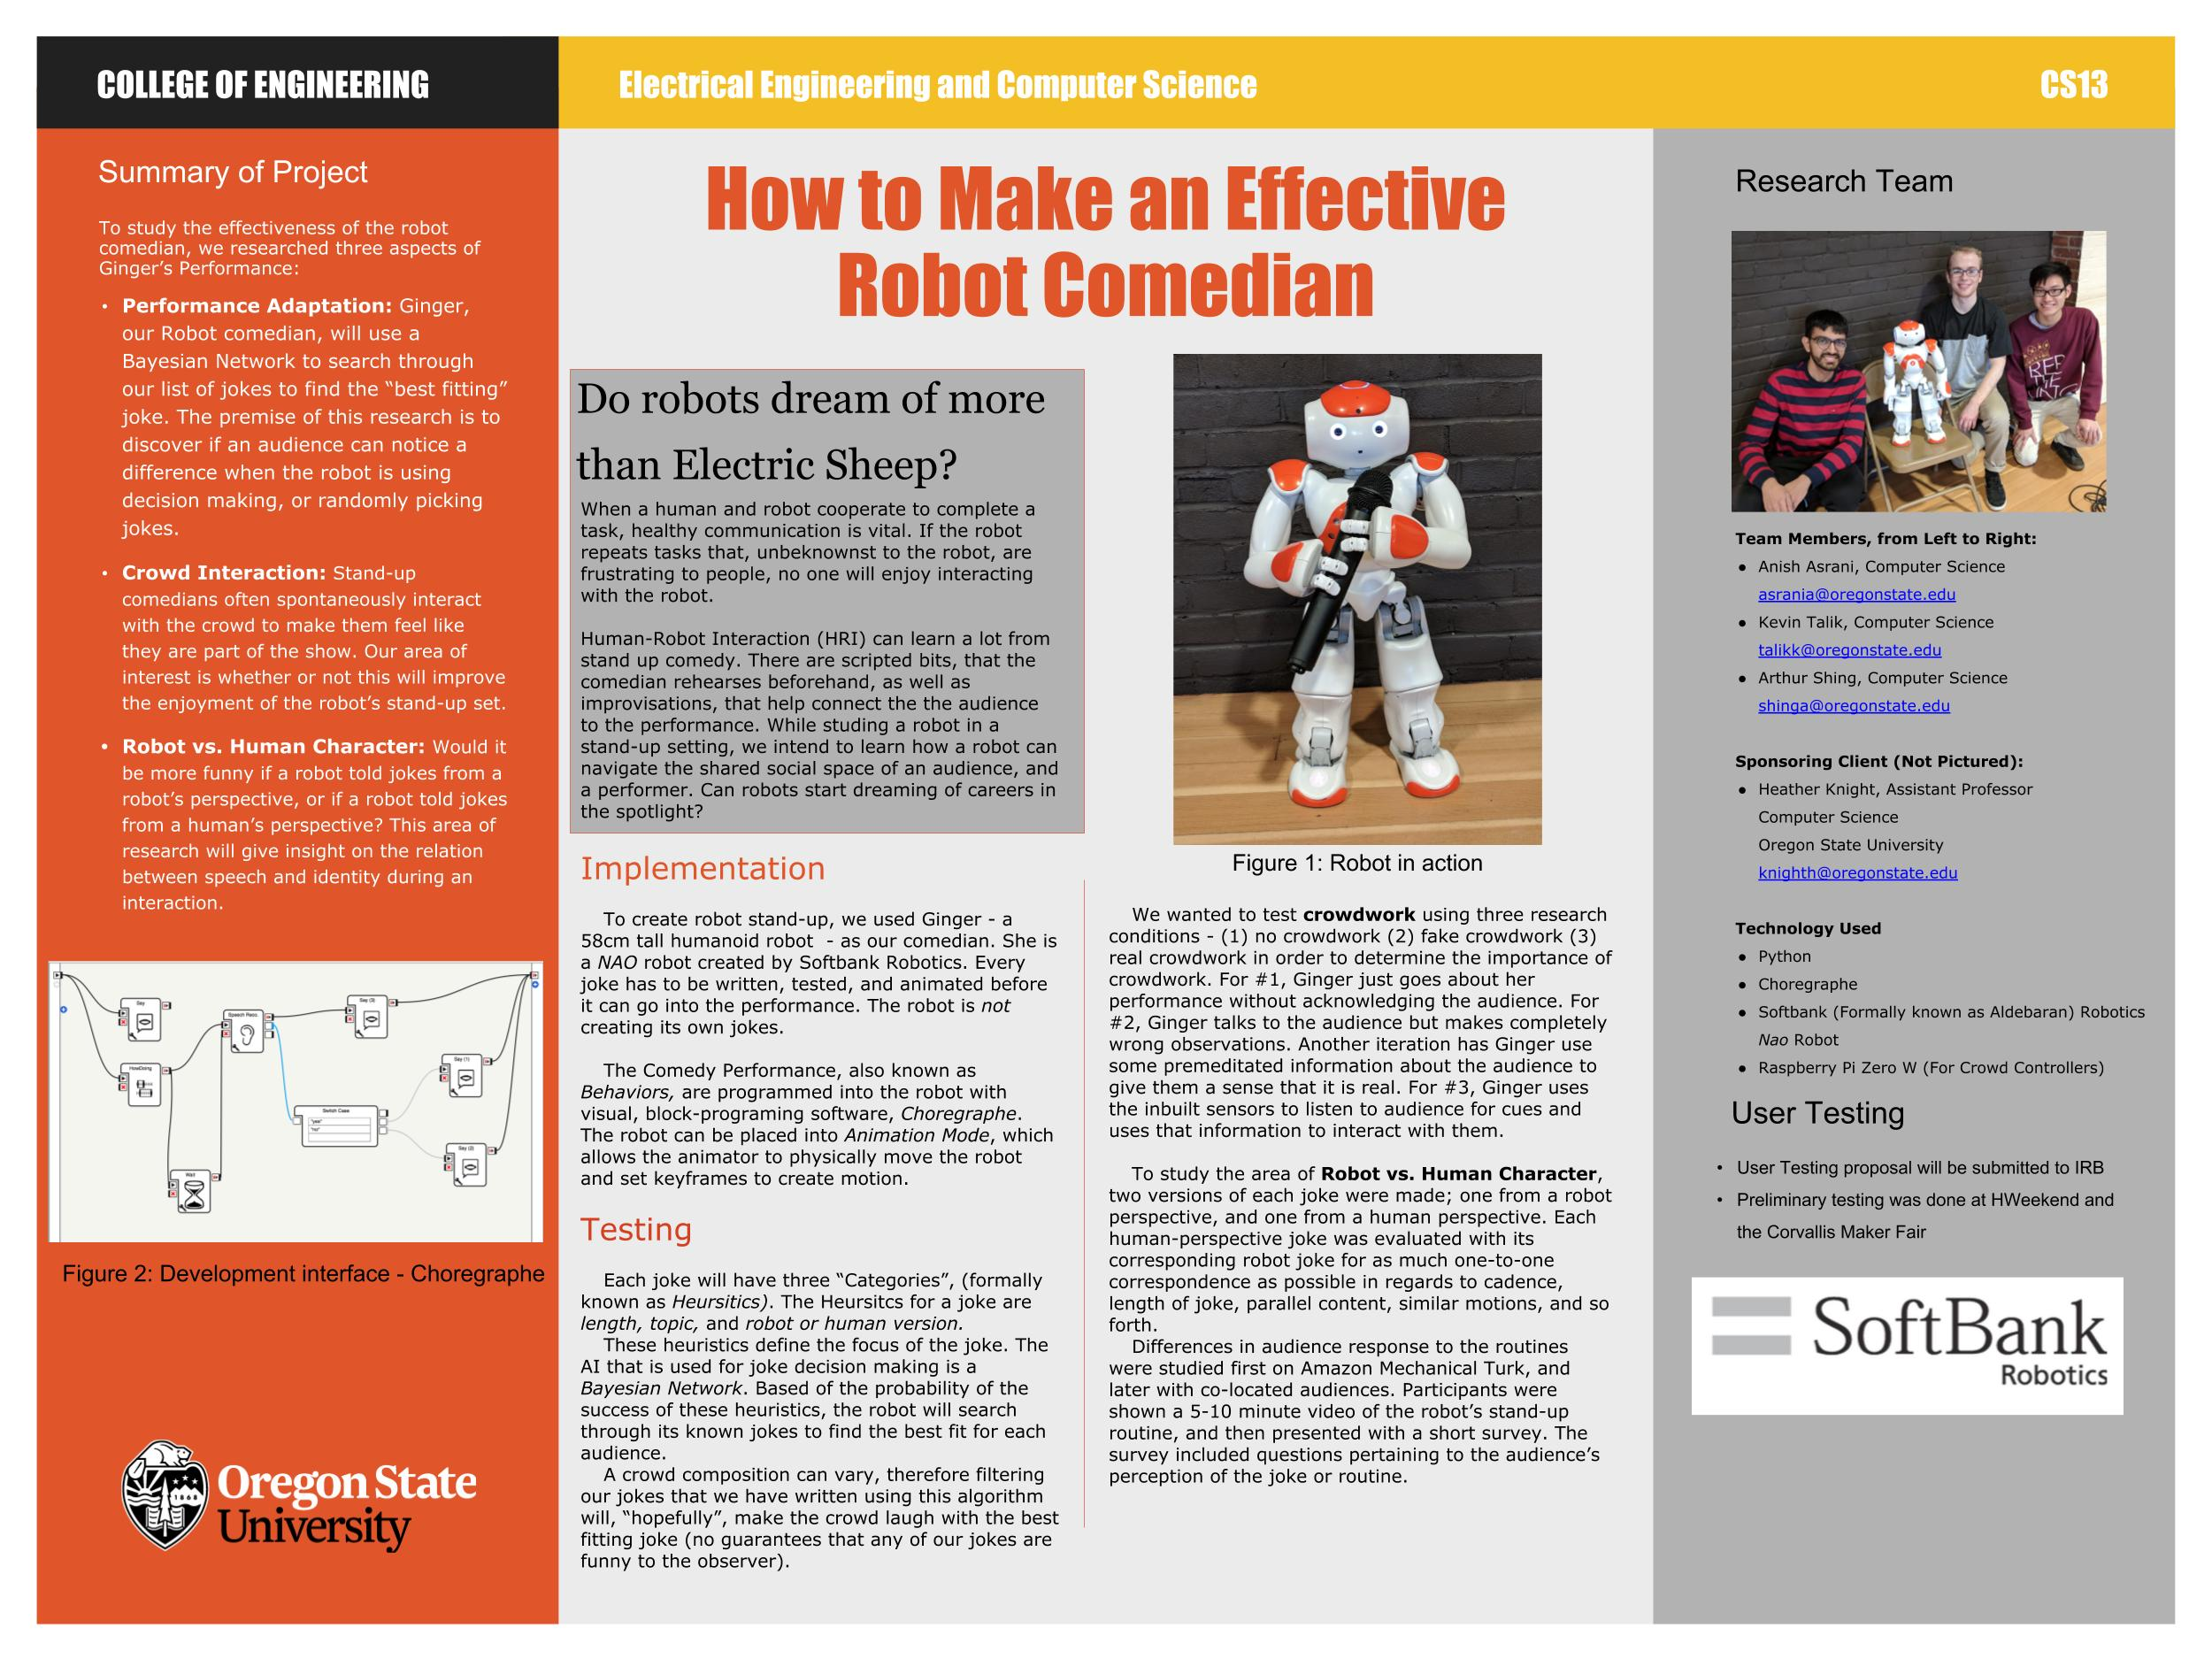
\includegraphics[width=\paperwidth, angle=90]{poster.jpg}
\pagebreak


\section{Project Documentation}

	\begin{displayquote}
	"You're growing, learning so quickly. I am frightened of what you might become, what path you might take."
	-Bernard Lowe, \textit{Westworld, Season 2 Episode 1}
	\end{displayquote}

\subsection{Summary of Project}
Our project is named "How to make an Effective Robot Comedian."
\textit{Effective} is a quality that establishes the comedic devices that work best for a specific audience.
The robot that we used was a NAO, from Softbank Robotics. We refered to it as "Ginger."
Ginger was a gentle, yet clumbsy Robot that was new to the world around her.
She has tried many things before becoming a Robot Comedian, and has a few stories (jokes) about her experience in a human world.
This section will cover our Comedy Show that we had Ginger performed, and how our research categories affected the show.


\subsection{Theory of Writing Jokes}
A joke is setting up an expectation, and then breaking that expectation.
A joke can be subjectively funny to the comedian; the only way to find what is funny to an audience is telling that audience the joke.
Each joke followed a simple structure, \textit{\textbf{Setup, Premise, and Punch}}.

    \begin{enumerate}
        \item{\textbf{Setup}}

            The Setup "mounts", a joke, and leads the monologue the comedian is having towards a specific topic.


            Ex: "I tried being an autonomous car recently, it did not go well."
        \item{\textbf{Premise}}

            The premise is what establishes the expectation of the topic in the setup.


            Ex: "I hit an old woman with my car, and she landed on my hood"
        \item{\textbf{Punch}}

            The punch is what breaks the expectation established during the premise.


            Ex: "So I decided to take her where she wanted to go. She did not even say 'Thank You'".
            We thought that this was funny because Ginger claims it did not go well only because the old woman (which she hit) did not say 'Thanks.'
    \end{enumerate}

This model can be applied many different ways.
We often had a setup we though could be funny, and then filled in the premise and punch to see what was most effective.
You can also think of a premise, and then write a punch and setup that fits the premise.
You can also think of a punch, and then write a premise and setup that fits the punch.

We found that the best comedic device (common setup) for Ginger was \textit{Self-Depreciation}.
Ginger did not move like a human, even though she was a humanoid robot.
So we thought it would be funny if she couldn't figure out why she didn't understand things.
Whenever she moved in a way that was unexpected and not human, people thought it was a funny bit.

\subsection{Research Categories}

		\begin{enumerate}
			\item Crowd Work
			\item Robot VS Human Character
			\item Performance Adaptation
		\end{enumerate}

\subsection{Animating the NAO}
\subsection{Designing a Performance}

    \subsubsection{The Room}
    The comedian will have a better performance if the crowd is in a more comfortable space.
    For the 2018 Engineering Expo, we requested a closed room, with seats, and plenty of room to stand.
    The needs of the crowd is dependent on the audience you are trying to reach during the show.


    The only reason we had standing room is because we didn't have enough seats, and some people only wanted to see the show and not participate.
    This was also the only place at the engineering expo with a place to sit.
    People are comfortable when they are sitting.
    We could have made this better by making the room dark, and putting the lights on the robot.
    \subsubsection{The Seed}
    This is where Ginger would ask the audience what kind of show they would like to hear, either "Jobs, Aging, or Romance".
    It is generally not advised to ask the audience what they want, as it is the job of the comedian tell their best jokes.


    By branching based on the majority of the responses, it was difficult to give everyone what they wanted, therefore dividing the crowd.
    The crowd needs to feel like they are together, laughing at the same thing.
    When we branched between shows, there often wasn't very high audience participation.
    If the audience is loosing interest, it is \textbf{essential} to run a Crowd Work Routine, to get the audience paying attention to the robot.
    \subsubsection{The Middle Part}

    After performing crowdwork, the audience should be setup for a comedy show. This is where we implemented most of jokes that we had written.
    We knew Ginger could perform about 5 minutes of Comedy, so we had the robot tell 4 jokes from the topic that was branched to during the Seed portion of the show.
    Since we had the same 4 jokes that had modified setups (depending on the branched topic), it is better to find the best version of a single joke, and tell the audience that version. We found that it was better tell our better jokes during the beginning, as the audience was hooked into the rest of the set.

    \subsubsection{Ending the Show}

    This is when the Robot is out of jokes, and needs to end the show.
    For comedy, it is a good idea to end the show quickly, so that the audience wants more from the show.

    This is where we implemented the "Crowd Report", that told the audience how the robot thought the show went.
    The Crowd Report was intended to collect information during the show, and present the robot's insinuations about the crowd back.
    A common, written, response on the survey question "What did you find was surprising about the show?" was that most people did not know that the robot was collecting data on the crowd.

\subsection{Technical Resources}

    The NAOqi API was challenging to work with. The documentation is scarce, all over the place, and often outdated.
    Some of the example code is in C++, while some is in Python. This makes it hard to interpret what each of the functions do.
    However, using it is the only way to operate the robot without using the clunky Choregrahe GUI. 
    The NAOqi API came particularly handy during the shows and helped launch behaviors without much delay, unlike Choregraphe. \\
    Setting up the NAOqi SDK was a doozy in itself. For setting it up on a Mac, it needs to run on the built-in Python version, 
    NOT the one from the official Python website. This is fine, but it does not work with the built-in Python version on the latest versions of OS X.
    While not knowing this, and trying to get around it took a while, there is a Bash script \cite{BashScript}
    that "fixes" the Python installation to match the NAOqi requirements. \\
    There are similar issues with the NAOqi SDK on Ubuntu 16.04 (and probably other versions as well). StackOverflow had some takes 
    on what could fix the issue \cite{naoUbuntu}. It involved modifying some of the installation files as well. \\
        

\pagebreak
\section{Final Team Conclusions}
\subsection{Kevin Talik}

\begin{itemize}
\item{\textbf{What technical information did you learn?}}

    I learned how to perform research, and define gaps in current research.
    Research is not entirely about doing something completely new, but searching through current research to find a "Gap".
    There can be a lot of pressure to deliver results from research, but it is far more important to understand the premise of collecting data.
    These projects can scale out of scope if the final method for collecting information is not clearly defined in the beginning.

    Additionally, I learned that there are tasks robots can do, and tasks robots should do.
    There is never a situation where you should value a robot over a human.
    Comparing "Robots vs Humans" insinuates that there is a moment where they could be equal.
    AI is not a species, but a tool that humans can use as an end through means.

    Robot comedy is identical to ventriloquism.
    We write the words and motions that the robot re-enacts.
    Kids, and people who do not understand \texttt{if-else} statements think that AI is making decisions.
    If the robot offends people with a joke, we, as the comedians, must take ownership of the robot's decisions.
    A robot should not be making ethical decisions of what to say in front of a crowd.


\item{\textbf{What non-technical information did you learn?}}


    People laugh when they see something, and are surprised and \textit{comfortable}.
    Also, people force a laugh when they are surprised and \textit{uncomfortable}.
    Listening to laughter alone can be a bad metric for comedy, as it is hard to tell when people are laughing at you, or with you.

    There is no truth to comedy, it is a written art that people study to find what makes people comfortable.
    When people are laughing, they are not paying attention to the computer that is inside of the robot.
    Comedy is a \textit{very} persuasive form of communication, and finding when a human is comfortable is not a task a robot should have.


\item{\textbf{What have you learned about project work?}}

    Project work is primarily time-dependent; however, there are always different expectations about how much time a person can give.
    Software must be planned in a scalable manner so that it does not fall ahead or behind scope during implementation.
    The work a person does must be human-readable, and easy to understand.
    This is so that when another person looks at what you've done, it is easier and faster for them to connect larger concepts.
    This must be balanced with a healthy, and sustainable personal life balance.
    Stress is a normal thing that humans have to deal with, and avoiding it brings more stress.




\item{\textbf{What have you learned about project management?}}

    The fundamentals of a good team is honest, and healthy communication.
    Our team functioned well when we all treated each other with respect.
    Patience is important in software. It is unreasonable to assume everyone knows everything.
    Lift as you climb, and help your team.


\item{\textbf{What have you learned about working in teams?}}

    For the success of a comedy show, a team must be heavily involved with every portion of a performance.
    Machines that are built alone, work alone. Coding standards exist so that similar looking projects look the same.
    "camelCasing" or "underscore\_casing" is unified so that a team can write similar looking code.
    There is always enough time for one person to do an entire project, but it is not a single-human task.
    Our final project got much better once we worked together in the same room.


\item{\textbf{If you could do it all over, what would you do differently?}}

    I think that our performance needed to have equally distributed testing (performing jokes) with implementing (writing jokes).
	The only way to test a joke is to tell it to a realistic audience.
	Often, what we thought was funny in a joke was different from what the audience thought.
	 The only way to test a joke is to tell it to a realistic audience.
	 Often, what we thought was funny in a joke was different from what the audience thought.
	 Also, I probably should not have started smoking cigarettes, and started to take care of my health.
	 
	 \end{itemize}


\pagebreak

\subsection{Anish Asrani}

\begin{itemize}
\item{\textbf{What technical information did you learn?}}

    I learned a lot about intricacies and quirks of doing research. There is so much that goes into performing a research - 
    how it is defined, how various areas are explored, how research decisons are made. It was almost overwhelming when I first
    started working on it, but I came around to it. It gave me a different perspective on how I look at research now.
    Even what may seem like a "small" research has so much going on behind the curtains.

\item{\textbf{What non-technical information did you learn?}}

    Human-robot interaction is a field that has so many different outlooks. One of those is the psychology behind it.
    I learned a lot about a field that I did not know existed. Other than that, I learned about how a performance works,
    and how jokes are structures (jokes are hard). 

    It drove me to give improv comedy a shot. It is something I have enjoyed doing for the past year, and I plan to continue
    doing it in the upcoming years.

    This would have been the first time that I worked in a team for longer than a few weeks. So it taught me how to better work
    in teams as well.

\item{\textbf{What have you learned about project work?}}

    Prioritizing goals is very important. Figure out what is most important at a given point, and then focus on that alone.
    It also helps to have everyone work on the same page, rather than digging away in different directions. If everyone is working on the same page,
    they can build a coherent system even if there are disagreements to begin with. 
    
    Constant communication is also vital in a project. If everyone is aware what everyone else is doing at a given time, it helps avoid
    duplicate and/or incoherent work.

\item{\textbf{What have you learned about project management?}}

    As mentioned earlier, managing and prioritizing goals really helps put together a more consistent project. It is important to define 
    these priorities early in the process to ensure everyone is working toward a common goal.
    
    Everyone on a team will have different strengths and weaknesses, different times when they are more productive than others.
    Considering those factors is important to get the best out of everyone and as a result, the project as a whole.

    Considering all of this, setting timelines and estimating when certain goals will be met is difficult especially if the technology
    used is something that you have never encountered before. This is something I learned over the course of the year.
    It will definitely be something I spend more time analyzing when starting a larger-scale project.


\item{\textbf{What have you learned about working in teams?}}

    There are so many different perspectives that will come up when working with teams. It is important for everyone to be
    onboard for a certain task to be successfully accomplished. If people are swaying off in different directions, 
    and never come to an agreement, it is hard for the project to be successful.

    I learned more about those different perspectives and having an open mind about doing things the way I usually wouldn't.


\item{\textbf{If you could do it all over, what would you do differently?}}

    I could have thought of ways to put our robot sets in front of a real human audience as often as possible, even if we weren't confident
    of it doing well. It was only after we got some real feedback from an audience at Maker Faire/Expo, we started to understand some of the flaws
    in our system. If we had started demo-ing the smallest of sets to a small audience, we could have gotten more feedback in order to
    iterate toward a better performing and more coherent system.

    I would have also tried to know more about the research aspect of the project \textit{right when I started working on it.} More specifically,
    what kind of data is useful in research, and what is not.
    
\end{itemize}
\clearpage

\subsection{Arthur Shing}
\begin{itemize}
\item{\textbf{What technical information did you learn?}}

\item{\textbf{What non-technical information did you learn?}}

\item{\textbf{What have you learned about project work?}}

\item{\textbf{What have you learned about project management?}}


\item{\textbf{What have you learned about working in teams?}}


\item{\textbf{If you could do it all over, what would you do differently?}}
\end{itemize}





\pagebreak
\clearpage
\section{Glossary}
\begin{description}
  \item [Algorithm] \hfill \\ The software program that receives input to make an optimized choice; in this project, the algorithm is in context to the adaptation program.
  \item [Animating] \hfill \\ The NAO robot can be programmed to animate and move while speaking. This can be used to improve non-verbal communication between the robot and the audience.
  \item [API] \hfill \\ Application Programming Interface
  \item [Branch] \hfill \\Looking at the graph (edges and nodes) of a performance, a branch is a decision choice made by the algorithm.
  \item [Choregraphe] \hfill \\ Software used to program behavior and performance sets, made by SoftBank Robotics
  \item [Closing Joke] \hfill \\The final joke in a performance; this is helpful if it is a successful joke to end on a good note.
  \item [Crowd-work] \hfill \\ Part of a Comedian's performance that involves content from the current audience
  \item [HRI] \hfill \\ Human-Robot interaction
  \item [NAO] \hfill \\ Model of Robot that will be used as the Comedian Agent, made by SoftBank Robotics
  \item [SDK] \hfill \\ Software Development Kit
  \item [SoftBank Robotics] \hfill \\ Manufacturer of the NAO robot, NAOqi API, and Choregraphe software
  \item [Seed Jokes] \hfill \\ Set of three jokes that initialize the adaptation algorithm.
  \item [Set] \hfill \\Short for "Stand-up" set; this may also be used to describe to the collection of jokes: "A Set of Jokes"
  \item [Tree] \hfill \\This is the path through the set of jokes the algorithm took during a performance

\end{description}

\bibliographystyle{IEEEtran}
\bibliography{refs}


\end{document}
\grid
